% supplement.tex -- Supplementary material for the CJFAS manuscript (manuscript.tex)
% Compile with: latexmk -pdf supplement.tex   (biblatex + biber)
% Tables S1--S7 and S9--S13 were generated from the result CSV files named in their captions.
\documentclass[11pt,letterpaper,fleqn]{article}
\usepackage[T1]{fontenc}
\usepackage[utf8]{inputenc}
\usepackage{lmodern}
\usepackage[margin=1in]{geometry}
\usepackage{setspace}
\usepackage{amsmath}
\setlength{\mathindent}{0pt}
\usepackage{graphicx}
\usepackage{booktabs}
\usepackage{tabularx}
\usepackage{array}
\usepackage{etoolbox}
\usepackage{adjustbox}
\usepackage[labelfont=bf,labelsep=period,font=small,justification=raggedright,singlelinecheck=false]{caption}
\usepackage[english]{babel}
\usepackage{csquotes}
\usepackage[style=authoryear,backend=biber,maxcitenames=2,mincitenames=1,maxbibnames=99,
  giveninits=true,uniquename=false,uniquelist=false,dashed=false,doi=true,url=true,
  isbn=false,eprint=false,sorting=nyt,date=year,useprefix=true]{biblatex}
\usepackage[hidelinks]{hyperref}
% --- approximation of the CJFAS (Harvard, author-year) reference style -------------------
% In text: (Bundy and Fanning 2005), (Frank et al. 2011). In the list:
% Bundy, A., and Fanning, L.P. 2005. Title. Journal, 62(7): 1474--1489. doi:10.1139/f05-086.
\DeclareNameAlias{sortname}{family-given}
\DeclareNameAlias{default}{family-given}
\renewrobustcmd*{\bibinitdelim}{}
\DeclareDelimFormat{nameyeardelim}{\addspace}
\DeclareDelimFormat[bib,biblist]{finalnamedelim}{\addcomma\addspace\bibstring{and}\space}
\DeclareDelimFormat[bib,biblist]{multinamedelim}{\addcomma\space}
\renewbibmacro*{date+extradate}{%
  \iffieldundef{labelyear}{}{\printtext{\printlabeldateextra}}}
\DeclareFieldFormat*{title}{#1\isdot}
\DeclareFieldFormat{journaltitle}{#1}
\DeclareFieldFormat[article]{volume}{#1}
\DeclareFieldFormat[article]{number}{\mkbibparens{#1}}
\DeclareFieldFormat{pages}{#1}
\renewcommand*{\bibpagespunct}{\addcolon\space}
\renewbibmacro*{in:}{}
\renewbibmacro*{volume+number+eid}{%
  \printfield{volume}\printfield{number}\setunit{\addcomma\space}\printfield{eid}}
\renewbibmacro*{journal+issuetitle}{%
  \usebibmacro{journal}\setunit*{\addcomma\space}%
  \iffieldundef{series}{}{\newunit\printfield{series}\setunit{\addspace}}%
  \usebibmacro{volume+number+eid}\setunit{\addspace}\usebibmacro{issue+date}%
  \setunit{\addcolon\space}\usebibmacro{issue}\newunit}
\DeclareFieldFormat{doi}{doi\addcolon\href{https://doi.org/#1}{\nolinkurl{#1}}}
\DeclareFieldFormat{url}{\url{#1}}
\DeclareFieldFormat{urldate}{}
\AtEveryBibitem{\clearfield{month}\clearfield{issn}\clearlist{language}\clearfield{urlyear}}
% internal bookkeeping notes in references.bib are not printed
\DeclareSourcemap{\maps[datatype=bibtex]{
  \map{\step[fieldsource=note, match=\regexp{^(Closest|A\sversion|R\spackage|Report\sof|Read\sas|Scanned|English\sedition|Published\sMarch)}, final]
       \step[fieldset=note, null]}}}
\DeclareSortingNamekeyTemplate{\keypart{\namepart{prefix}}\keypart{\namepart{family}}\keypart{\namepart[inits]{given}}}
\setcounter{biburllcpenalty}{7000}
\setcounter{biburlucpenalty}{8000}
\setcounter{biburlnumpenalty}{8000}
\addbibresource{references.bib}

\onehalfspacing
\renewcommand{\thesection}{S\arabic{section}}
\renewcommand{\thetable}{S\arabic{table}}
\renewcommand{\thefigure}{S\arabic{figure}}
\renewcommand{\theequation}{S\arabic{equation}}
\AtBeginEnvironment{table}{\singlespacing}
\newcolumntype{L}{>{\raggedright\arraybackslash}X}
\newcommand{\yr}{yr$^{-1}$}
\makeatletter\g@addto@macro\UrlBreaks{\do\_}\makeatother
\newcommand{\gm}{g\,m$^{-2}$}
\begin{document}
\sloppy

\begin{center}
{\large\bfseries Supplementary material for}\\[0.5em]
{\Large\bfseries A weak, conditional trap: a size-spectrum test of predator--prey role reversal as the cause of non-recovery of Atlantic Cod on the eastern Scotian Shelf\par}
\vspace{1em}
[AUTHOR NAME(S) -- PLACEHOLDER]
\end{center}

\noindent Contents: S1 model equations and settings; S2 calibration procedure; S3 the earlier model versions v1 and v2; S4 additional results; S5 departures from the rule that scenarios differ only in fishing and initial state; S6 code, data and reproducibility. Supplementary Tables~S1--S14 and Figs.~S1--S8 follow the text. Every number in these tables is read from the result files named in the captions (paths relative to the project repository).

% ---------------------------------------------------------------------------
\section{Model equations and settings}\label{sec:S-eq}

The model is the multispecies size-spectrum model of mizer \autocite{scott2014mizer,delius2013mizer}, version 3.4.0.9003, created with defaults edition~3. In that edition the sums over the predation kernel are evaluated by fast Fourier transforms on a zero-padded grid (so that the kernels of planktivores with large predator:prey mass ratios do not wrap around the grid), and the size dynamics use a second-order scheme with a van Leer flux limiter and bin-averaged integrals. Units are g~m$^{-2}$ of shelf and years; 1~\gm{} = 110~kt over $1.1\times10^{5}$~km$^{2}$ \autocite{dfo2010greyseals}.

\paragraph{Size spectra.} The abundance density $N_i(w,t)$ of species $i$ at body mass $w$ obeys
\begin{equation}
\frac{\partial N_i}{\partial t}+\frac{\partial (g_i N_i)}{\partial w}=-\mu_i N_i ,\qquad g_i(w_0)N_i(w_0)=R_i ,
\end{equation}
with egg mass $w_0=1$~mg for all species. The grid has 120 logarithmically spaced bins from 1~mg to 20~kg; the resource grid extends down to about $10^{-6}$~g. The time step is 0.1~yr (semi-implicit Euler).

\paragraph{Encounter and feeding.} The encounter rate is
\begin{equation}
E_i(w)=\gamma_i w^{q}\int \phi_i(w/w')\Big[N_R(w')+\sum_j \theta_{ij}N_j(w')\Big]w'\,\mathrm{d}w',\qquad
\phi_i(x)=\exp\!\left[-\frac{\ln^{2}\!\big(x/\beta_i\big)}{2\sigma_i^{2}}\right],
\end{equation}
with $q=0.717$, the kernel parameters $\beta_i$, $\sigma_i$ of main-text Table~1 and the interaction matrix $\theta_{ij}$. All $\theta_{ij}=1$ except $\theta_{ij}=s$ for $i\in\{$herring, sand lance, Capelin$\}$ and $j\in\{$cod, Haddock, Silver Hake, American Plaice$\}$. The feeding level is $f_i=E_i/(E_i+h_iw^{n})$ with $n=2/3$. The energy available for growth and reproduction is $\alpha f_i h_i w^{n}-k_{s,i}w^{p}$ with $\alpha=0.6$ and $p=0.7$; a size-dependent proportion $\psi_i(w)$, zero for immature fish and rising through maturation to one at the asymptotic size, goes to reproduction and the rest to growth $g_i$. The search-volume coefficient $\gamma_i$ is set so that small individuals have feeding level $f_0=0.6$, and $h_i$ and $k_{s,i}$ were calibrated so that each species reaches maturity at its age at maturity (Section~S2).

\paragraph{Mortality.} The total mortality rate is
\begin{equation}
\mu_i(w)=\sum_j\int \theta_{ji}\,\phi_j(w'/w)\,(1-f_j(w'))\,\gamma_j w'^{q}\,N_j(w')\,\mathrm{d}w' + z_{0,i}+\mu_{\mathrm{bg},i}(w)+F_i(w),
\end{equation}
the sum of predation by the modelled fish, a constant external mortality $z_{0,i}=0.6\,w_{\infty,i}^{-1/3}$ (mizer default; 0.025~\yr{} for cod), the background early-life mortality $\mu_{\mathrm{bg},i}$ of main-text eq.~1 and fishing $F_i(w)$. The background term equals 0.5 times the reference specific growth rate (growth at feeding level $f_0$ before reproduction), tapered by $1/(1+(w/1\,\mathrm{g})^{2})$; it is computed from the species parameters and held fixed, and recomputed whenever growth parameters change during calibration. A ratio of 1 was tried first: the forage fish and American Plaice then needed reproductive efficiencies above 1 to sustain the targets. A purely size-based rate (a power law in body mass, the same for all species) was also tried and rejected: in the model the larvae of the small, slow-maturing species (sand lance, Capelin, American Plaice) grow several times more slowly than cod larvae, and the same size-based rate removed them.

\paragraph{Reproduction.} Density-independent egg production is $R_{\mathrm{di},i}=\frac{\epsilon_i}{2w_0}\int\psi_i(\alpha f_ih_iw^{n}-k_{s,i}w^{p})N_i\,\mathrm{d}w$, with reproductive efficiency $\epsilon_i$, and recruitment follows the Beverton--Holt form $R_i=R_{\max,i}R_{\mathrm{di},i}/(R_{\max,i}+R_{\mathrm{di},i})$. The reproduction level is $R_i/R_{\max,i}$ at the steady state; setting it leaves the steady state unchanged and changes only the strength of density dependence away from it.

\paragraph{Resource.} The plankton--benthos resource follows semichemostat dynamics,
\begin{equation}
\frac{\partial N_R(w)}{\partial t}=r(w)\big(c(w)-N_R(w)\big)-\mu_R(w)N_R(w),\qquad c(w)=\kappa w^{-\lambda}\ (w<10\,\mathrm{g}),
\end{equation}
with $\lambda=2.05$, $\kappa=3$ and $r(w)=1.41\,w^{-0.22}$~\yr{}. The rate was fitted through two production:biomass ratios from \textcite{bundy2004mass}: 8.4~\yr{} for \textit{Calanus finmarchicus} (about 0.3~mg) and 3.04~\yr{} for euphausiids (about 30~mg). When it was set, the capacity was rebalanced so that the steady state did not change. In v2, with the same resource parameters, the standing resource biomass was 32~\gm{} below 1~mg and 16~\gm{} between 1 and 100~mg (\nolinkurl{results/v2/baseline_zooplankton_vs_bundy.csv}), compared with copepod biomass of 30--34~\gm{} and large-zooplankton biomass of 9 (independent estimate) to 16~\gm{} (Ecopath) in \textcite{bundy2004mass}.

\paragraph{Fishing.} Gears and their selectivities are in Table~\ref{tab:S-gear} and the effort history in Table~\ref{tab:S-effort}. Catchability is 1 for every gear--species pair, so effort equals fishing mortality on fully selected sizes. Baseline (1980--85 steady state) efforts are cod 0.40, Haddock, Silver Hake and American Plaice 0.30 each, and pelagic 0.10~\yr{}.

% ---------------------------------------------------------------------------
\section{Calibration procedure}\label{sec:S-calib}

\paragraph{Stage 1 (v2 procedure, $s=1$).} The model was built with \texttt{newMultispeciesParams()} from the species, gear and interaction tables, with the background mortality set as an external-mortality array. Growth was matched to age at maturity and single-species steady states found (\texttt{matchGrowth()}, \texttt{steadySingleSpecies()}), baseline fishing was switched on, and \texttt{matchBiomasses()}, \texttt{matchGrowth()} and \texttt{tuneSteadyState()} were iterated, keeping the best fixed point with all reproductive efficiencies below 1. This is the v2 calibration (Section~\ref{sec:S-versions}).

\paragraph{Stage 2 (v3).} The v3 biomass targets (main-text Table~1) were set, the resource rate $r(w)$ imposed, and $s$ stepped from 1 to 5, 10 and 20. At each step, all seven biomass targets were solved simultaneously. The unknowns were the log factors by which each species' spectrum is scaled; the residuals were the log ratios of modelled to target biomass above the survey cut-off. Each evaluation scaled the spectra and re-settled the model with \texttt{tuneSteadyState(solver = "project")}, which holds recruitment and resource fixed; the maximum recruitment was effectively unlimited during calibration. The system was solved by Newton's method with a finite-difference Jacobian (step 0.05 on the log scale), step halving and a trust region of at most a factor 4.5 per step. Newton solutions alternated with a rescaling of the growth parameters $\gamma_i$, $h_i$ and $k_{s,i}$ by the ratio of modelled to target age at maturity, after which the background mortality was recomputed. This rescaling is what \texttt{matchGrowth()} does, but without its final \texttt{steadySingleSpecies()} call, which in this model moved a steady state far from where it was (recorded in the project's notes on possible mizer issues; not yet reported upstream). At the end the Beverton--Holt reproduction levels were imposed, which leaves the steady state unchanged. The resulting biomass errors are below 0.6\%, ages at maturity within 0.5\% and reproductive efficiencies at most 0.049 (main-text Table~2). Simpler loops (\texttt{matchBiomasses()} followed by \texttt{tuneSteadyState()}) oscillated in this strongly coupled model. Newton solves of \texttt{tuneSteadyState()} occasionally failed inside the van Leer limiter and then fell back to projection.

\paragraph{Forage reproduction level.} The leading eigenvalue of the linearised dynamics around the calibrated state (\texttt{getStability()}) becomes positive when the forage reproduction level falls below 0.120. The level was fitted on a logit scale by one-dimensional minimisation of $[\ln(\text{forage ratio}/7.87)]^{2}$ for the documented-fishing hindcast, restricted to $[0.170, 0.95]$, i.e.\ at least 0.05 above the critical value. The fit ended on the lower bound (0.171), where the hindcast forage ratio is 1.36 (\nolinkurl{results/hindcast_calibration.csv}).

\paragraph{Variants.} For the sensitivity analysis, each $s$ in $\{1, 5, 10, 40\}$ was recalibrated from the calibrated model by the same Newton procedure with $s$ stepped geometrically from 20, and accepted if the maximum biomass error was below 15\% and all reproductive efficiencies were below 1 (achieved errors 0.7--1.7\%; Table~\ref{tab:S-map}). For $s=80$ and 160 the evaluations stopped settling, and a first attempt had not finished after 25 minutes, so these were run with $s$ changed in the main model and are flagged as not recalibrated. The 200-bin model for the numerical check was rebuilt from the calibrated species parameters, interaction matrix, gears and resource (interpolated onto the new grid) and recalibrated by the same procedure (maximum error 1.0\%).

% ---------------------------------------------------------------------------
\section{The earlier model versions}\label{sec:S-versions}

Both earlier versions are kept unchanged in the project repository (scripts in \nolinkurl{R/v1} and \nolinkurl{R/v2}, results in \nolinkurl{results/v1} and \nolinkurl{results/v2}). Both used purely size-based predation by forage fish on young groundfish ($s=1$). Main-text Table~3 compares the three versions; Table~\ref{tab:S-versions} gives their calibrations.

\paragraph{v1: a conventional calibration.} v1 had the same species, life history, kernels and size grid as v3. The resource had $\kappa=1.4$ and a replenishment rate of $2w^{-1/3}$~\yr{}. There was no explicit early-life background mortality, the reproduction levels were 0.5 (cod), 0.75 (other groundfish) and 0.5 (forage fish), and three gears (cod, other groundfish, pelagic) were used. Biomasses matched their targets within 2.3\%. Under the historical fishing trajectory, cod fell only to 0.30 of its baseline SSB in 1993 and regained 50\% one year later (\nolinkurl{results/v1/hindcast_metrics.csv}); forage-fish biomass peaked at 1.50 times baseline between 1993 and 2025. Forage fish killed 2.0\% of cod between 1~mg and 0.1~g (\nolinkurl{results/v1/baseline_cod_early_life.csv}). From the baseline and from the 1993 state, cod converged to the same equilibrium (3.89 times baseline SSB), and rare cod invaded the cod-free community at $+0.23$~\yr{} (Fig.~\ref{fig:S-v1}). With $s$ raised without recalibration, $s=30$ (forage fish eating 45\% of cod 1~mg--0.1~g at baseline) delayed 50\% recovery to 12 years after 1993, and $s=100$ (87\%) to 90 years, but the cod-free state was still invadable ($+0.12$~\yr{}; \nolinkurl{results/v1/sensitivity.csv}). v1 could not test the hypothesis. Beverton--Holt reproduction levels of 0.5 limited how far forage recruitment could rise, cod early life was almost free of modelled mortality (cod reproductive efficiency $5.6\times10^{-5}$ hid the rest), and the plankton was barely depleted (resource level 0.98--0.99 at $10^{-5}$--$10^{-3}$~g; \nolinkurl{results/v1/baseline_resource_level.csv}).

\paragraph{v2: plankton constraint, explicit early-life mortality and a forced boom.} v2 introduced the resource parameters and the background mortality used in v3. It also introduced low reproduction levels (0.1 for groundfish; 0.284 for forage fish, calibrated to the boom) and one gear per groundfish species. To reproduce the observed post-collapse community without assuming why it arose, the other groundfish were driven by effective mortalities fitted to their survey declines: Haddock 0.88 and 0.98, Silver Hake 1.54 and 1.33, American Plaice 2.40 and 2.88~\yr{} in 1986--2004 and from 2005 (\nolinkurl{results/v2/hindcast_calibration*.csv}). In the calibration run only, cod was held near its survey level by an effective $F$ of 6.28 from 1994. The calibration was loose: cod biomass was 61\% and American Plaice 59\% above target, and the modelled cod yield was 115~kt against landings of 53.5~kt (Table~\ref{tab:S-versions}). The forced run produced a forage boom of 9.40 (Fig.~\ref{fig:S-v2hind}), but the boom did not fade (13.3 in 2005--12, against 4.11 observed). In the boom year 2000 forage fish killed 4.3\% of cod between 1~mg and 1~g (0.29\% at baseline). Cod survival over that range fell from 2.41\% to 1.63\%, by a factor of 0.93 from higher mortality and 0.73 from slower growth. From the model's version of the observed 2000 community, cod regained 50\% of baseline SSB in 7 years under the moratorium, with or without either pathway (\nolinkurl{results/v2/pathways_diagnostic_metrics.csv}). The cod-free community (forage fish 19 times baseline) was invaded at $+0.52$~\yr{}. With $s$ raised without recalibration, a failure to recover for 32 years or more required $s\approx11.8$ and an alternative state $s\approx18.9$ (\nolinkurl{results/v2/sensitivity_thresholds.csv}; Fig.~\ref{fig:S-v2sens}). At those values, however, the uncalibrated model could no longer sustain the 1980s cod: equilibrium cod at baseline fishing fell to 62\% ($s=10$) and 8\% ($s=20$) of the calibrated value (\nolinkurl{results/v2/sensitivity.csv}). This is why v3 recalibrates the baseline with $s$ in place.

% ---------------------------------------------------------------------------
\section{Additional results}\label{sec:S-results}

\paragraph{Baseline.} Fig.~\ref{fig:S-baseline} adds the feeding levels and the resource depletion to main-text Fig.~1; Table~\ref{tab:S-budget} gives the pre-recruit mortality budgets for the four groundfish, and Table~\ref{tab:S-resource} the resource levels and consumption at baseline and in the 2000 state of run~B.

\paragraph{Hindcast detail.} Fig.~\ref{fig:S-hind} shows the groups and individual species against the survey and the resource bands for runs A, A0 and B. In run~A the other groundfish declined after about 2000 as cod rose to several times its baseline biomass; in run~B they increased.

\paragraph{Forage fishing.} Tables~\ref{tab:S-ffgrid} and \ref{tab:S-altgrid} list every programme from the modelled collapsed 2025 state and from the alternative stable state; Table~\ref{tab:S-equil} and Fig.~\ref{fig:S-forage} give the constant-$F$ equilibria. At forage-fish $F=0$ with cod $F=0.02$, the equilibrium from the baseline had cod at 7.35 times baseline SSB, whereas from the collapsed state cod remained absent with forage fish at 26.5 times baseline (not converged after 500 years).

\paragraph{Sensitivity and numerical checks.} Table~\ref{tab:S-oat} gives the one-at-a-time variants and the cod collapse $F$ for each $s$, Table~\ref{tab:S-map} the full map over $s$ and the forage reproduction level (summarised in main-text Table~4 and Fig.~5), Fig.~\ref{fig:S-sens} the corresponding figure produced by the analysis script, Table~\ref{tab:S-hyst} the hysteresis sweep and Table~\ref{tab:S-numerical} and Fig.~\ref{fig:S-num} the numerical checks.

\paragraph{Conditional map.} Table~\ref{tab:S-condmap} extends the conditional test of the main text to 150 imposed starting states: five values of $s$, five boom sizes and six levels of cod depletion. For $s\leq10$ every start recovered for good, in at most 29 years, even with a 16-fold boom and cod at 0.1\% of its 1980s SSB. At $s=20$ every start recovered with a boom of fourfold or less. With the survey-sized boom (7.87), cod stayed down when it started at 2\% of its 1980s SSB or less; with a boom twice that size, at 4\% or less. At $s=40$ cod stayed down even from 10\% with booms of fourfold or more, but that variant's 1980s baseline is unstable, so these cells are not reliable.

% ---------------------------------------------------------------------------
\section{Departures from the scenario rule}\label{sec:S-departures}

The scenarios were designed to differ only in fishing effort and initial state. Table~\ref{tab:S-departures} lists every departure, where it is used and why. No artificial fishing mortality is used anywhere in v3.

% ---------------------------------------------------------------------------
\section{Code, data and reproducibility}\label{sec:S-code}

All analyses were run in R 4.6.2 with mizer 3.4.0.9003, ggplot2 4.0.3, patchwork 1.3.2, dplyr 1.2.1 and tidyr 1.3.2. The main model (v3) is produced by the following scripts, run from the repository root:
\begin{itemize}\setlength{\itemsep}{0pt}
\item \nolinkurl{R/functions.R}: model construction, calibration (\texttt{calibrate\_v3n()}, \texttt{solve\_biomasses()}, \texttt{scale\_growth()}), scenario runner (\texttt{run\_scenario()}), invasion test, elevated adult mortality (\texttt{elevate\_M()}), pre-recruit budgets.
\item \nolinkurl{R/00_fishbase_lookup.R}: FishBase extraction (optional; cached in \nolinkurl{data/fishbase/}).
\item \nolinkurl{R/01_build_model.R}: calibration and calibration checks; \nolinkurl{R/02_collapse_moratorium.R}: hindcasts A, A0, B and pathway diagnostics; \nolinkurl{R/03_bistability.R}: two starts, invasion, hysteresis; \nolinkurl{R/04_forage_fishing_recovery.R}, \nolinkurl{R/04b_forage_fishing_from_alternative_state.R}, \nolinkurl{R/04c_observed_like_start.R}: forage fishing and the conditional test; \nolinkurl{R/05_sensitivity.R}; \nolinkurl{R/06_numerical_checks.R}; \nolinkurl{R/07_adult_mortality_alternative.R}.
\item \nolinkurl{R/run_all.R}: driver; with the calibration caches in place the nine v3 scripts ran in 61 minutes.
\item \nolinkurl{R/09_paper_figures.R}: main-text Figs.~1--3 and 5--7, drawn from the result files only.
\item \nolinkurl{R/08_website_data.R}: additional runs for a policy explorer web page with the same scenario runner, including the conditional map of Table~\ref{tab:S-condmap} (stored in \nolinkurl{website/data/site_data.json}; 355 overlapping runs reproduce the result files above exactly, \nolinkurl{website/data/sanity_checks.csv}).
\end{itemize}
Inputs are in \nolinkurl{data/v3/} (species, gear, interaction and effort tables), outputs in \nolinkurl{results/} (CSV) and \nolinkurl{figures/}, and saved models (\texttt{saveParams()}) in \nolinkurl{models/}. Supplementary Figs.~S1--S8 are the figures written by the analysis scripts themselves, reproduced unchanged.

\clearpage
% ---------------------------------------------------------------------------
\printbibliography[title={References}]

\clearpage

\begin{table}[p]\caption{Fishing mortality (\yr{}) on fully selected sizes by gear in the hindcast (\nolinkurl{data/v3/effort_history.csv}). Each value applies from the year given until the next row. Cod values are stylised from landings and survey SSB \autocite{fanning2003assessment}, $F$ above $F_{\max}$ in 1988--92 \autocite{mohn1994assessment} and post-closure estimates \autocite{mohn2012laurentian}; other values are assumptions.}\label{tab:S-effort}
\centering\small\begin{adjustbox}{max width=\textwidth}\begin{tabular}{@{}rrrrrrl@{}}\toprule
From & Cod & Haddock & Silver Hake & American Plaice & Pelagic & Note\\\midrule
1970 & 0.4 & 0.3 & 0.3 & 0.3 & 0.1 & baseline 1970s\\
1980 & 0.45 & 0.35 & 0.35 & 0.35 & 0.1 & 1980-85\\
1986 & 0.7 & 0.45 & 0.45 & 0.45 & 0.1 & 1986-89\\
1990 & 1.1 & 0.55 & 0.55 & 0.55 & 0.1 & 1990-92\\
1993 & 0.3 & 0.3 & 0.3 & 0.3 & 0.1 & 1993 (cod moratorium from Sept)\\
1994 & 0.02 & 0.2 & 0.2 & 0.2 & 0.1 & moratorium: cod bycatch 0.02; other groundfish reduced\\
2025 & 0.02 & 0.2 & 0.2 & 0.2 & 0.1 & end of hindcast\\
\bottomrule\end{tabular}\end{adjustbox}\end{table}
\begin{table}[p]\caption{Fishing gears (\nolinkurl{data/v3/gear_params.csv}): logistic length selectivity with 50\% and 25\% selection at $L_{50}$ and $L_{25}$; catchability 1, so effort equals fishing mortality on fully selected sizes. Selectivities are assumptions. The observed cod yield (0.486~\gm{}~yr$^{-1}$ = 53.5~kt~yr$^{-1}$, the 1980--85 mean landings in \citeauthor{fanning2003assessment} \citeyear{fanning2003assessment}) was used as a check.}\label{tab:S-gear}
\centering\small\begin{adjustbox}{max width=\textwidth}\begin{tabular}{@{}llrrr@{}}\toprule
Gear & Species & $L_{50}$ (cm) & $L_{25}$ (cm) & Catchability\\\midrule
cod & Atlantic Cod & 40 & 35 & 1\\
haddock & Haddock & 35 & 31 & 1\\
silver hake & Silver Hake & 25 & 22 & 1\\
plaice & American Plaice & 30 & 27 & 1\\
pelagic & Atlantic Herring & 20 & 18 & 1\\
pelagic & Northern Sand Lance & 10 & 9 & 1\\
pelagic & Capelin & 11 & 10 & 1\\
\bottomrule\end{tabular}\end{adjustbox}\end{table}
\begin{table}[p]\caption{Pre-recruit mortality budgets (eq.~2 of the main text) at the 1980--85 baseline for the four groundfish, and for cod in the 2000 state of run~B (adult cod $M$ 0.8 from 1990). Integral, $\int\mu_k/g\,\mathrm{d}w$ by source; killed, percentage of the cohort killed by each source; share, forage-fish share of all deaths in the window (\nolinkurl{results/baseline_prerecruit_budget.csv}, \nolinkurl{results/pathways_cod_prerecruit_budget.csv}).}\label{tab:S-budget}
\centering\footnotesize\begin{adjustbox}{max width=\textwidth}\begin{tabular}{@{}llrrrrrrrr@{}}\toprule
 & & & & \multicolumn{3}{c}{Mortality integral} & \multicolumn{2}{c}{\% of cohort killed} & Forage share\\\cmidrule(lr){5-7}\cmidrule(lr){8-9}
Species / state & Window & Survival (\%) & Duration (yr) & forage & groundfish & background & forage & background & of deaths (\%)\\\midrule
Cod, baseline & 1 mg--1 g & 2.08 & 0.39 & 0.217 & 0.098 & 3.55 & 5.8 & 91.5 & 5.9\\
Cod, baseline & 1 mg--10 g & 1.13 & 0.93 & 0.241 & 0.479 & 3.74 & 5.9 & 91.9 & 5.9\\
Haddock, baseline & 1 mg--1 g & 2.10 & 0.37 & 0.207 & 0.094 & 3.55 & 5.6 & 91.7 & 5.7\\
Haddock, baseline & 1 mg--10 g & 1.14 & 0.89 & 0.230 & 0.459 & 3.74 & 5.6 & 92.1 & 5.7\\
Silver Hake, baseline & 1 mg--1 g & 2.02 & 0.40 & 0.226 & 0.102 & 3.54 & 6.0 & 91.2 & 6.1\\
Silver Hake, baseline & 1 mg--10 g & 1.05 & 0.97 & 0.250 & 0.499 & 3.74 & 6.1 & 91.5 & 6.1\\
American Plaice, baseline & 1 mg--1 g & 1.43 & 0.81 & 0.453 & 0.205 & 3.55 & 11.4 & 86.0 & 11.6\\
American Plaice, baseline & 1 mg--10 g & 0.48 & 1.96 & 0.502 & 1.004 & 3.74 & 11.4 & 86.2 & 11.5\\
Cod, run B 2000 & 1 mg--1 g & 1.47 & 0.39 & 0.545 & 0.089 & 3.58 & 13.0 & 85.1 & 13.2\\
Cod, run B 2000 & 1 mg--10 g & 0.74 & 0.94 & 0.607 & 0.502 & 3.77 & 13.1 & 85.4 & 13.1\\
\bottomrule\end{tabular}\end{adjustbox}\end{table}
\begin{table}[p]\caption{Resource (plankton and benthos) level, the ratio of abundance to carrying capacity, and the share of resource production eaten by fish, at the 1980--85 baseline and in the 2000 state of run~B (\nolinkurl{results/pathways_resource_level.csv}). Lower rows: decomposition of the change in cod survival between the two states into mortality and growth effects (\nolinkurl{results/pathways_survival_decomposition.csv}).}\label{tab:S-resource}
\centering\small\begin{adjustbox}{max width=\textwidth}\begin{tabular}{@{}rrrrr@{}}\toprule
Resource body mass (g) & Level, baseline & Level, run B 2000 & \% eaten, baseline & \% eaten, run B 2000\\\midrule
1e-05 & 0.989 & 0.980 & 1.1 & 1.9\\
0.0001 & 0.984 & 0.968 & 1.6 & 3.1\\
0.001 & 0.982 & 0.961 & 1.8 & 3.9\\
0.01 & 0.974 & 0.954 & 2.6 & 4.6\\
0.1 & 0.915 & 0.914 & 8.5 & 8.6\\
1 & 0.716 & 0.716 & 28.4 & 28.4\\
5 & 0.574 & 0.550 & 42.6 & 45.0\\
\midrule
Cod survival from 1 mg to & Baseline (\%) & Run B 2000 (\%) & Mortality effect & Growth effect\\\midrule
1 g & 2.08 & 1.47 & $\times$0.73 & $\times$0.97\\
10 g & 1.13 & 0.74 & $\times$0.68 & $\times$0.97\\
\bottomrule\end{tabular}\end{adjustbox}\end{table}
\begin{table}[p]\caption{Forage-fishing programmes from the modelled collapsed 2025 state (run~B in 2025 with baseline parameters; cod $F$ 0.02; other gears at moratorium levels; projections to 2125; \nolinkurl{results/forage_fishing_grid.csv}). $D$, programme duration (100 = permanent); $F=0.1$ is the status quo. Years are counted from the start of the programme. Persistent: SSB $\geq50$\% of baseline in each of the last 30 years.}\label{tab:S-ffgrid}
\centering\scriptsize\begin{adjustbox}{max width=\textwidth}\begin{tabular}{@{}rrrrcrrrr@{}}\toprule
Forage $F$ & $D$ (yr) & Years to 50\% & Years to 100\% & Persistent & Cod SSB 2125 & Min.\ forage & Forage yield during & Cod yield 2026--85\\
 & & SSB & SSB & & / baseline & / baseline & programme (kt yr$^{-1}$) & (kt)\\\midrule
0.1 & 5 & 39 & 44 & yes & 6.20 & 0.021 & 23 & 132\\
0.25 & 5 & 41 & 45 & yes & 5.34 & 0.0070 & 46 & 117\\
0.5 & 5 & 42 & 46 & yes & 4.39 & 0.0019 & 70 & 103\\
0.75 & 5 & 42 & 47 & yes & 4.24 & $7.3\times10^{-4}$ & 85 & 95\\
1 & 5 & 43 & 48 & yes & 4.22 & $3.5\times10^{-4}$ & 96 & 92\\
1.5 & 5 & 43 & 48 & yes & 4.20 & $1.0\times10^{-4}$ & 115 & 88\\
2 & 5 & 43 & 48 & yes & 4.20 & $3.8\times10^{-5}$ & 134 & 87\\
3 & 5 & 43 & 48 & yes & 4.20 & $7.7\times10^{-6}$ & 173 & 86\\
0.25 & 10 & 41 & 46 & yes & 4.62 & 0.0030 & 36 & 108\\
0.5 & 10 & 43 & 47 & yes & 4.22 & $3.9\times10^{-4}$ & 45 & 93\\
0.75 & 10 & 43 & 48 & yes & 4.20 & $9.2\times10^{-5}$ & 48 & 89\\
1 & 10 & 43 & 48 & yes & 4.20 & $2.7\times10^{-5}$ & 52 & 88\\
1.5 & 10 & 43 & 48 & yes & 4.20 & $3.1\times10^{-6}$ & 59 & 87\\
2 & 10 & 43 & 48 & yes & 4.20 & $4.7\times10^{-7}$ & 68 & 86\\
3 & 10 & 43 & 48 & yes & 4.20 & $1.8\times10^{-8}$ & 87 & 86\\
0.25 & 15 & 42 & 46 & yes & 4.36 & 0.0015 & 29 & 103\\
0.5 & 15 & 43 & 48 & yes & 4.21 & $1.1\times10^{-4}$ & 31 & 91\\
0.75 & 15 & 43 & 48 & yes & 4.20 & $1.5\times10^{-5}$ & 33 & 88\\
1 & 15 & 43 & 48 & yes & 4.20 & $2.5\times10^{-6}$ & 35 & 87\\
1.5 & 15 & 43 & 48 & yes & 4.20 & $9.8\times10^{-8}$ & 39 & 87\\
2 & 15 & 43 & 48 & yes & 4.20 & $5.8\times10^{-9}$ & 45 & 86\\
3 & 15 & 43 & 48 & yes & 4.20 & $4.2\times10^{-11}$ & 58 & 86\\
0.25 & 20 & 42 & 47 & yes & 4.28 & $8.5\times10^{-4}$ & 24 & 99\\
0.5 & 20 & 43 & 48 & yes & 4.20 & $3.5\times10^{-5}$ & 24 & 90\\
0.75 & 20 & 43 & 48 & yes & 4.20 & $2.5\times10^{-6}$ & 25 & 88\\
1 & 20 & 43 & 48 & yes & 4.20 & $2.3\times10^{-7}$ & 26 & 87\\
1.5 & 20 & 43 & 48 & yes & 4.20 & $3.1\times10^{-9}$ & 30 & 87\\
2 & 20 & 43 & 48 & yes & 4.20 & $6.9\times10^{-11}$ & 34 & 86\\
3 & 20 & 43 & 48 & yes & 4.20 & $9.4\times10^{-14}$ & 43 & 86\\
0.25 & 30 & 42 & 47 & yes & 4.23 & $3.1\times10^{-4}$ & 17 & 97\\
0.5 & 30 & 43 & 48 & yes & 4.20 & $3.5\times10^{-6}$ & 16 & 90\\
0.75 & 30 & 43 & 48 & yes & 4.20 & $7.1\times10^{-8}$ & 16 & 88\\
1 & 30 & 43 & 48 & yes & 4.20 & $1.9\times10^{-9}$ & 17 & 87\\
1.5 & 30 & 43 & 48 & yes & 4.20 & $3.0\times10^{-12}$ & 20 & 87\\
2 & 30 & 43 & 48 & yes & 4.20 & $9.8\times10^{-15}$ & 23 & 86\\
3 & 30 & 43 & 48 & yes & 4.20 & $4.7\times10^{-19}$ & 29 & 86\\
0.25 & 100 & 42 & 47 & yes & 4.20 & $6.1\times10^{-6}$ & 5 & 97\\
0.5 & 100 & 43 & 48 & yes & 4.20 & $8.7\times10^{-11}$ & 5 & 90\\
0.75 & 100 & 43 & 48 & yes & 4.20 & $5.3\times10^{-16}$ & 5 & 88\\
1 & 100 & 43 & 48 & yes & 4.20 & $4.9\times10^{-21}$ & 5 & 87\\
1.5 & 100 & 43 & 48 & yes & 4.20 & $4.7\times10^{-30}$ & 6 & 87\\
2 & 100 & 43 & 48 & yes & 4.20 & $5.2\times10^{-38}$ & 7 & 86\\
3 & 100 & 43 & 48 & yes & 4.20 & $4.0\times10^{-52}$ & 9 & 86\\
\bottomrule\end{tabular}\end{adjustbox}\end{table}
\begin{table}[p]\caption{Forage-fishing programmes from the model's alternative stable state (cod-free equilibrium at cod $F=0$; cod and the other groundfish reintroduced at $10^{-3}$ of baseline; cod $F$ 0.02; 150 years; \nolinkurl{results/forage_fishing_alt_state_grid.csv}). $D=150$ is permanent; $F=0.1$ is the status quo. --, 50\% of baseline SSB not reached.}\label{tab:S-altgrid}
\centering\scriptsize\begin{adjustbox}{max width=\textwidth}\begin{tabular}{@{}rrrcrrrrr@{}}\toprule
Forage $F$ & $D$ (yr) & Years to 50\% & Persistent & Cod SSB end & Other groundfish & Min.\ forage & Forage yield during & Cod yield, first\\
 & & SSB & & / baseline & end / baseline & / baseline & programme (kt yr$^{-1}$) & 60 yr (kt)\\\midrule
0.1 & 5 & -- & no & $2.82\times10^{-4}$ & $3.2\times10^{-18}$ & 19 & 580 & 1\\
0.25 & 5 & -- & no & $4.28\times10^{-4}$ & $4.3\times10^{-18}$ & 13 & 1169 & 2\\
0.5 & 5 & -- & no & 0.00150 & $1.2\times10^{-17}$ & 7.4 & 1749 & 6\\
0.75 & 5 & -- & no & 0.00403 & $3.4\times10^{-17}$ & 4.7 & 2103 & 14\\
1 & 5 & -- & no & 0.00922 & $8.0\times10^{-17}$ & 3.1 & 2365 & 27\\
1.5 & 5 & 18 & no & 0.0538 & $3.6\times10^{-16}$ & 1.4 & 2799 & 88\\
2 & 5 & 16 & yes & 6.55 & $2.2\times10^{-10}$ & 0.63 & 3217 & 335\\
3 & 5 & 16 & yes & 6.55 & $2.3\times10^{-7}$ & 0.14 & 4117 & 711\\
0.25 & 10 & -- & no & $9.52\times10^{-4}$ & $7.5\times10^{-18}$ & 13 & 1043 & 4\\
0.5 & 10 & -- & no & 0.0120 & $7.3\times10^{-17}$ & 6.7 & 1359 & 31\\
0.75 & 10 & 18 & yes & 1.34 & $1.5\times10^{-15}$ & 3.6 & 1461 & 170\\
1 & 10 & 16 & yes & 6.55 & $3.7\times10^{-8}$ & 1.8 & 1496 & 704\\
1.5 & 10 & 16 & yes & 6.56 & $2.0\times10^{-7}$ & 0.42 & 1556 & 669\\
2 & 10 & 17 & yes & 6.56 & $1.9\times10^{-7}$ & 0.084 & 1680 & 576\\
3 & 10 & 17 & yes & 6.56 & $1.4\times10^{-7}$ & 0.0040 & 2075 & 462\\
0.25 & 15 & -- & no & 0.00211 & $1.3\times10^{-17}$ & 13 & 999 & 6\\
0.5 & 15 & 20 & yes & 6.55 & $1.3\times10^{-13}$ & 1.8 & 1208 & 196\\
0.75 & 15 & 17 & yes & 6.55 & $1.3\times10^{-7}$ & 1.8 & 1196 & 741\\
1 & 15 & 17 & yes & 6.56 & $1.6\times10^{-7}$ & 1.3 & 1133 & 668\\
1.5 & 15 & 17 & yes & 6.56 & $1.6\times10^{-7}$ & 0.12 & 1070 & 540\\
2 & 15 & 17 & yes & 6.56 & $1.2\times10^{-7}$ & 0.0088 & 1127 & 452\\
3 & 15 & 17 & yes & 6.55 & $7.5\times10^{-8}$ & $7.3\times10^{-5}$ & 1384 & 414\\
0.25 & 20 & -- & no & 0.00468 & $2.4\times10^{-17}$ & 13 & 979 & 11\\
0.5 & 20 & 20 & yes & 6.55 & $2.8\times10^{-8}$ & 1.8 & 1123 & 685\\
0.75 & 20 & 17 & yes & 6.56 & $1.1\times10^{-7}$ & 1.2 & 1031 & 662\\
1 & 20 & 17 & yes & 6.56 & $1.2\times10^{-7}$ & 0.43 & 908 & 584\\
1.5 & 20 & 17 & yes & 6.56 & $1.1\times10^{-7}$ & 0.011 & 808 & 458\\
2 & 20 & 17 & yes & 6.56 & $8.1\times10^{-8}$ & $2.1\times10^{-4}$ & 845 & 420\\
3 & 20 & 17 & yes & 6.53 & $5.6\times10^{-8}$ & $1.7\times10^{-7}$ & 1038 & 414\\
0.25 & 30 & -- & no & 0.0270 & $8.4\times10^{-17}$ & 13 & 959 & 31\\
0.5 & 30 & 20 & yes & 6.55 & $4.1\times10^{-8}$ & 1.4 & 941 & 603\\
0.75 & 30 & 17 & yes & 6.56 & $7.2\times10^{-8}$ & 0.12 & 736 & 558\\
1 & 30 & 17 & yes & 6.56 & $7.6\times10^{-8}$ & 0.0091 & 615 & 479\\
1.5 & 30 & 17 & yes & 6.55 & $6.2\times10^{-8}$ & $2.2\times10^{-5}$ & 539 & 426\\
2 & 30 & 17 & yes & 6.53 & $5.0\times10^{-8}$ & $5.4\times10^{-8}$ & 564 & 419\\
3 & 30 & 17 & yes & 4.87 & $3.1\times10^{-7}$ & $1.7\times10^{-12}$ & 692 & 414\\
0.25 & 150 & 40 & yes & 5.63 & $3.7\times10^{-11}$ & 1.1 & 399 & 135\\
0.5 & 150 & 20 & yes & 4.52 & $4.3\times10^{-9}$ & 0.24 & 220 & 490\\
0.75 & 150 & 17 & yes & 4.21 & $2.8\times10^{-8}$ & $5.1\times10^{-6}$ & 148 & 467\\
1 & 150 & 17 & yes & 4.21 & $8.0\times10^{-8}$ & $2.1\times10^{-13}$ & 123 & 448\\
1.5 & 150 & 17 & yes & 4.21 & $2.0\times10^{-7}$ & $9.9\times10^{-28}$ & 108 & 426\\
2 & 150 & 17 & yes & 4.21 & $2.6\times10^{-7}$ & $4.9\times10^{-41}$ & 113 & 419\\
3 & 150 & 17 & yes & 4.21 & $3.1\times10^{-7}$ & $1.0\times10^{-62}$ & 138 & 414\\
\bottomrule\end{tabular}\end{adjustbox}\end{table}
\begin{table}[p]\caption{Long-run equilibria at constant forage-fish $F$ with cod $F$ 0.02 or 0.40 (other gears at moratorium levels), from the baseline and from the modelled collapsed 2025 state; up to 500 years (\nolinkurl{results/forage_fishing_equilibria.csv}). Converged: largest relative rate of change $<5\times10^{-4}$~\yr{}. Feeding level and weight at age 5 refer to a cod individual even where cod is absent.}\label{tab:S-equil}
\centering\scriptsize\begin{adjustbox}{max width=\textwidth}\begin{tabular}{@{}rrlcrrrrrr@{}}\toprule
Forage $F$ & Cod $F$ & Start & Conv. & Cod SSB & Forage & Other groundfish & Forage yield & Feeding level & Cod weight\\
 & & & & / baseline & / baseline & / baseline & (kt yr$^{-1}$) & 1-kg cod & age 5 (kg)\\\midrule
0 & 0.02 & baseline & yes & 7.35 & 2.50 & $3.7\times10^{-10}$ & 0 & 0.60 & 1.28\\
0 & 0.02 & collapsed & no & $1.25\times10^{-8}$ & 26.5 & $6.1\times10^{-49}$ & 0 & 0.85 & 1.75\\
0 & 0.4 & baseline & yes & $2.08\times10^{-15}$ & 26.5 & $1.4\times10^{-9}$ & 0 & 0.85 & 1.75\\
0 & 0.4 & collapsed & yes & $6.13\times10^{-19}$ & 26.5 & $1.4\times10^{-9}$ & 0 & 0.85 & 1.75\\
0.1 & 0.02 & baseline & yes & 6.56 & 1.84 & $7.9\times10^{-10}$ & 49.4 & 0.57 & 1.19\\
0.1 & 0.02 & collapsed & yes & 6.56 & 1.84 & $1.7\times10^{-9}$ & 49.3 & 0.57 & 1.19\\
0.1 & 0.4 & baseline & yes & $3.29\times10^{-21}$ & 19.3 & $3.5\times10^{-12}$ & 580 & 0.84 & 1.90\\
0.1 & 0.4 & collapsed & yes & $1.82\times10^{-20}$ & 19.3 & $3.8\times10^{-10}$ & 580 & 0.84 & 1.90\\
0.25 & 0.02 & baseline & yes & 5.64 & 1.10 & $3.9\times10^{-13}$ & 71.5 & 0.53 & 1.08\\
0.25 & 0.02 & collapsed & no & 5.63 & 1.10 & $1.5\times10^{-25}$ & 71.4 & 0.53 & 1.08\\
0.25 & 0.4 & baseline & no & $4.98\times10^{-9}$ & $7.07\times10^{-19}$ & 2.4 & $4.91\times10^{-17}$ & 0.43 & 0.71\\
0.25 & 0.4 & collapsed & no & $1.27\times10^{-12}$ & $1.64\times10^{-18}$ & 2.4 & $1.14\times10^{-16}$ & 0.43 & 0.71\\
0.5 & 0.02 & baseline & yes & 4.52 & 0.237 & $1.4\times10^{-13}$ & 29.3 & 0.47 & 0.95\\
0.5 & 0.02 & collapsed & no & 4.22 & 0.00284 & $1.7\times10^{-21}$ & 0.349 & 0.45 & 0.91\\
0.5 & 0.4 & baseline & no & $4.85\times10^{-9}$ & $1.50\times10^{-50}$ & 2.4 & $2.03\times10^{-48}$ & 0.43 & 0.71\\
0.5 & 0.4 & collapsed & no & $1.16\times10^{-12}$ & $2.64\times10^{-50}$ & 2.4 & $3.56\times10^{-48}$ & 0.44 & 0.71\\
0.75 & 0.02 & baseline & yes & 4.21 & $1.29\times10^{-9}$ & $3.0\times10^{-10}$ & $2.32\times10^{-7}$ & 0.45 & 0.91\\
0.75 & 0.02 & collapsed & yes & 4.21 & $2.37\times10^{-21}$ & $7.0\times10^{-10}$ & $4.28\times10^{-19}$ & 0.45 & 0.91\\
0.75 & 0.4 & baseline & no & $4.76\times10^{-9}$ & $3.39\times10^{-79}$ & 2.4 & $6.68\times10^{-77}$ & 0.43 & 0.71\\
0.75 & 0.4 & collapsed & no & $1.14\times10^{-12}$ & $5.05\times10^{-79}$ & 2.4 & $9.94\times10^{-77}$ & 0.43 & 0.71\\
1 & 0.02 & baseline & yes & 4.21 & $7.24\times10^{-20}$ & $3.1\times10^{-10}$ & $1.71\times10^{-17}$ & 0.45 & 0.91\\
1 & 0.02 & collapsed & yes & 4.21 & $2.89\times10^{-34}$ & $7.1\times10^{-10}$ & $6.84\times10^{-32}$ & 0.45 & 0.91\\
1 & 0.4 & baseline & no & $4.68\times10^{-9}$ & $1.67\times10^{-105}$ & 2.4 & $4.27\times10^{-103}$ & 0.43 & 0.71\\
1 & 0.4 & collapsed & no & $1.10\times10^{-12}$ & $2.17\times10^{-105}$ & 2.4 & $5.53\times10^{-103}$ & 0.43 & 0.71\\
1.5 & 0.02 & baseline & yes & 4.21 & $3.63\times10^{-39}$ & $3.1\times10^{-10}$ & $1.24\times10^{-36}$ & 0.45 & 0.91\\
1.5 & 0.02 & collapsed & yes & 4.21 & $2.35\times10^{-58}$ & $7.1\times10^{-10}$ & $7.96\times10^{-56}$ & 0.45 & 0.91\\
1.5 & 0.4 & baseline & no & $4.70\times10^{-9}$ & $4.09\times10^{-152}$ & 2.4 & $1.48\times10^{-149}$ & 0.43 & 0.71\\
1.5 & 0.4 & collapsed & no & $1.09\times10^{-12}$ & $4.33\times10^{-152}$ & 2.4 & $1.56\times10^{-149}$ & 0.43 & 0.71\\
2 & 0.02 & baseline & yes & 4.21 & $6.65\times10^{-57}$ & $3.1\times10^{-10}$ & $2.88\times10^{-54}$ & 0.45 & 0.91\\
2 & 0.02 & collapsed & yes & 4.21 & $7.45\times10^{-79}$ & $7.1\times10^{-10}$ & $2.96\times10^{-76}$ & 0.45 & 0.91\\
2 & 0.4 & baseline & no & $4.72\times10^{-9}$ & $1.25\times10^{-192}$ & 2.4 & $5.70\times10^{-190}$ & 0.43 & 0.71\\
2 & 0.4 & collapsed & no & $1.08\times10^{-12}$ & $1.14\times10^{-192}$ & 2.4 & $5.17\times10^{-190}$ & 0.43 & 0.71\\
3 & 0.02 & baseline & yes & 4.21 & $8.62\times10^{-86}$ & $3.2\times10^{-10}$ & $4.78\times10^{-83}$ & 0.45 & 0.91\\
3 & 0.02 & collapsed & yes & 4.21 & $3.20\times10^{-114}$ & $7.1\times10^{-10}$ & $1.77\times10^{-111}$ & 0.45 & 0.91\\
3 & 0.4 & baseline & no & $4.55\times10^{-9}$ & $4.87\times10^{-262}$ & 2.4 & $3.00\times10^{-259}$ & 0.43 & 0.71\\
3 & 0.4 & collapsed & no & $1.03\times10^{-12}$ & $3.74\times10^{-262}$ & 2.4 & $2.31\times10^{-259}$ & 0.43 & 0.71\\
\bottomrule\end{tabular}\end{adjustbox}\end{table}

\begin{table}[p]\caption{Departures from the rule that scenarios differ only in fishing effort and initial state (main model v3).}\label{tab:S-departures}
\small\begin{tabularx}{\textwidth}{@{}p{0.33\textwidth}p{0.28\textwidth}L@{}}\toprule
Departure & Where used & Justification\\\midrule
Early-life vulnerability factor $s=20$ & all v3 runs & the assumption under test; the baseline was recalibrated with it\\
Forage reproduction level held at 0.171 & all v3 runs & the value fitted to the boom would make the 1980--85 state unstable (bound 0.05 above the critical 0.120)\\
Adult cod ($\geq$35~cm) natural mortality 0.8~\yr{} in 1990--2025 & run B; the adult-$M$ arm of the factorial; the collapsed 2025 state used as initial state in the bistability and forage-fishing tests & documented post-collapse $M$ \autocite{mohn2012laurentian}; labelled alternative, needed because documented fishing alone leaves cod uncollapsed\\
$s$ set to 1; resource held at baseline & pathway diagnostics; the $s=1$ arm of the factorial; $s=1$ runs of the conditional test & diagnostics only, not scenarios\\
Cod (and the other groundfish) reintroduced at $10^{-6}$ or $10^{-3}$ of baseline into the cod-free equilibrium & invasion test; forage fishing from the alternative state & tests of the alternative state\\
Imposed post-collapse community (survey ratios) as initial state & conditional test & initial state only\\
Cod reproduction level, resource productivity $\times0.5$ and $\times2$, forage reproduction levels, $s$ values (80, 160 without recalibration) & sensitivity analysis & sensitivity\\
\bottomrule\end{tabularx}\end{table}

\begin{table}[p]\caption{One-at-a-time sensitivity at $s=20$ (exact changes that leave the baseline unchanged; \nolinkurl{results/sensitivity_oat.csv}) and cod collapse $F$ for each $s$ (equilibrium SSB $<10$\% of baseline, cod $F$ in steps of 0.1 from 0.4, other gears at baseline; \nolinkurl{results/sensitivity_collapse_F.csv}). Run A, documented fishing; run B, plus adult cod $M$ 0.8 in 1990--2025.}\label{tab:S-oat}
\centering\scriptsize\begin{adjustbox}{max width=\textwidth}\begin{tabular}{@{}lrrrrrrl@{}}\toprule
Variant & Forage boom & Cod ratio & Years to 50\% & Run B: years & Invasion rate & Baseline & Outcome\\
 & (run A) & (run A) & from 1993 (A) & after 2025 & (\yr) & eigenvalue & \\\midrule
main model & 1.36 & 2.18 & 2 & 39 & -0.0099 & -0.0063 & alternative state exists, not reached\\
cod reproduction level 0.02 & 1.37 & 2.14 & 2 & 43 & -0.0108 & -0.0039 & alternative state exists, not reached\\
cod reproduction level 0.3 & 1.32 & 2.28 & 2 & 30 & -0.0066 & -0.0112 & alternative state exists, not reached\\
cod reproduction level 0.6 & 1.27 & 2.47 & 1 & 15 & +0.0033 & -0.0130 & recovers quickly ($\leq$ 20 yr)\\
resource productivity $\times$ 0.5 & 1.31 & 2.17 & 2 & 40 & -0.0175 & -0.0075 & alternative state exists, not reached\\
resource productivity $\times$ 2 & 1.40 & 2.19 & 2 & 39 & +0.2025 & -0.0055 & recovers quickly ($\leq$ 20 yr)\\
\midrule
$s$ & Recalibrated & Collapse $F$ & \multicolumn{2}{r}{SSB / baseline at $F=0.6$} & \multicolumn{2}{r}{SSB / baseline at $F=1.0$} & \\\midrule
1 & yes & 0.5 & \multicolumn{2}{r}{$8.1\times10^{-8}$} & \multicolumn{2}{r}{$9.9\times10^{-80}$} & \\
5 & yes & 0.5 & \multicolumn{2}{r}{$4.0\times10^{-8}$} & \multicolumn{2}{r}{$2.6\times10^{-14}$} & \\
10 & yes & 0.5 & \multicolumn{2}{r}{$7.6\times10^{-8}$} & \multicolumn{2}{r}{$5.2\times10^{-15}$} & \\
20 & yes & 0.5 & \multicolumn{2}{r}{$9.4\times10^{-23}$} & \multicolumn{2}{r}{$2.9\times10^{-55}$} & \\
40 & yes & 0.4 & \multicolumn{2}{r}{$7.7\times10^{-27}$} & \multicolumn{2}{r}{$3.0\times10^{-63}$} & \\
80 & no & 0.4 & \multicolumn{2}{r}{$2.7\times10^{-27}$} & \multicolumn{2}{r}{$1.0\times10^{-63}$} & \\
160 & no & 0.4 & \multicolumn{2}{r}{$5.2\times10^{-24}$} & \multicolumn{2}{r}{$2.0\times10^{-60}$} & \\
\bottomrule\end{tabular}\end{adjustbox}\end{table}
\begin{table}[p]\caption{Numerical checks (\nolinkurl{results/numerical_checks.csv}). The 200-bin model was rebuilt from the calibrated parameters and recalibrated to the same targets at $s=20$.}\label{tab:S-numerical}
\centering\scriptsize\begin{adjustbox}{max width=\textwidth}\begin{tabular}{@{}lrrlrrrrrrr@{}}\toprule
Case & Bins & $\Delta t$ (yr) & Method & Max.\ calib. & A: cod & A: forage & B: cod & B: years to 50\% & B + forage $F$ 1 & Invasion rate\\
 & & & & error (\%) & ratio & ratio & ratio & after 2025 & for 10 yr: years & (\yr; $R^2$)\\\midrule
reference & 120 & 0.1 & euler & 0.6 & 2.18 & 1.36 & 0.081 & 39 & 43 & -0.0099 (0.989)\\
short time step & 120 & 0.025 & euler & 0.6 & 2.16 & 1.37 & 0.076 & 41 & 44 & -0.0087 (0.987)\\
TR-BDF2 & 120 & 0.1 & tr-bdf2 & 0.6 & 2.16 & 1.36 & 0.075 & 41 & 45 & -0.0098 (0.989)\\
200 size bins & 200 & 0.1 & euler & 1.0 & 2.15 & 1.35 & 0.081 & 41 & 46 & -0.0169 (0.993)\\
\bottomrule\end{tabular}\end{adjustbox}\end{table}
\begin{table}[p]\caption{Hysteresis sweep in cod $F$ at baseline parameters with the other gears at moratorium levels (\nolinkurl{results/hysteresis.csv}). Each step was projected to equilibrium (largest relative rate of change $<5\times10^{-4}$~\yr{}) or for 400 years from the previous state; on the decreasing sweep cod was reset to $10^{-3}$ of its baseline biomass whenever it fell below that level. Biomasses relative to the 1980--85 baseline.}\label{tab:S-hyst}
\centering\scriptsize\begin{adjustbox}{max width=\textwidth}\begin{tabular}{@{}rrrcrrr|rrcrrr@{}}\toprule
\multicolumn{6}{c|}{Increasing $F$} & & \multicolumn{6}{c}{Decreasing $F$}\\
$F$ & Years & Conv. & Cod SSB & Forage & Other gf. & & $F$ & Years & Conv. & Cod SSB & Forage & Other gf.\\\midrule
0.0 & 150 & yes & 7.0 & 2.0 & $2.5\times10^{-9}$ & & 0.0 & 50 & yes & 4.4 & $1.5\times10^{-57}$ & $1.7\times10^{-10}$\\
0.1 & 75 & yes & 5.4 & 1.6 & $6.2\times10^{-11}$ & & 0.1 & 400 & no & 3.5 & $1.0\times10^{-52}$ & $1.4\times10^{-7}$\\
0.2 & 75 & yes & 4.5 & 1.7 & $5.1\times10^{-10}$ & & 0.2 & 275 & yes & 2.3 & $9.5\times10^{-30}$ & 0.56\\
0.3 & 400 & no & 1.7 & 0.54 & 0.44 & & 0.3 & 400 & no & 0.084 & $4.6\times10^{-24}$ & 2.4\\
0.4 & 400 & no & $6.8\times10^{-5}$ & $7.3\times10^{-9}$ & 2.1 & & 0.4 & 325 & yes & $4.7\times10^{-9}$ & $5.5\times10^{-27}$ & 2.4\\
0.5 & 400 & no & $1.8\times10^{-20}$ & $7.4\times10^{-30}$ & 2.4 & & 0.5 & 150 & yes & $3.6\times10^{-9}$ & $1.8\times10^{-29}$ & 2.4\\
0.6 & 400 & no & $3.1\times10^{-42}$ & $8.8\times10^{-43}$ & 2.4 & & 0.6 & 100 & yes & $3.2\times10^{-9}$ & $1.3\times10^{-30}$ & 2.4\\
0.7 & 400 & no & $9.0\times10^{-71}$ & $9.8\times10^{-40}$ & 2.4 & & 0.7 & 75 & yes & $3.6\times10^{-9}$ & $2.3\times10^{-31}$ & 2.4\\
0.8 & 100 & yes & $1.6\times10^{-79}$ & $5.7\times10^{-39}$ & 2.4 & & 0.8 & 75 & yes & $2.2\times10^{-10}$ & $6.2\times10^{-32}$ & 2.4\\
0.9 & 25 & yes & $4.3\times10^{-82}$ & $8.8\times10^{-39}$ & 2.4 & & 0.9 & 75 & yes & $1.6\times10^{-11}$ & $1.7\times10^{-32}$ & 2.4\\
1.0 & 25 & yes & $5.0\times10^{-85}$ & $1.4\times10^{-38}$ & 2.4 & & 1.0 & 50 & yes & $1.0\times10^{-9}$ & $4.5\times10^{-33}$ & 2.4\\
1.1 & 25 & yes & $2.7\times10^{-88}$ & $2.1\times10^{-38}$ & 2.4 & & 1.1 & 50 & yes & $2.1\times10^{-10}$ & $1.9\times10^{-33}$ & 2.4\\
1.2 & 25 & yes & $6.9\times10^{-92}$ & $3.3\times10^{-38}$ & 2.4 & & 1.2 & 50 & yes & $4.5\times10^{-11}$ & $7.7\times10^{-34}$ & 2.4\\
1.3 & 25 & yes & $8.7\times10^{-96}$ & $5.0\times10^{-38}$ & 2.4 & & 1.3 & 50 & yes & $1.1\times10^{-11}$ & $3.2\times10^{-34}$ & 2.4\\
1.4 & 25 & yes & $5.6\times10^{-100}$ & $7.8\times10^{-38}$ & 2.4 & & 1.4 & 50 & yes & $2.6\times10^{-12}$ & $1.3\times10^{-34}$ & 2.4\\
1.5 & 25 & yes & $1.9\times10^{-104}$ & $1.2\times10^{-37}$ & 2.4 & & 1.5 & 50 & yes & $6.9\times10^{-13}$ & $5.6\times10^{-35}$ & 2.4\\
1.6 & 25 & yes & $3.3\times10^{-109}$ & $1.9\times10^{-37}$ & 2.4 & & 1.6 & 50 & yes & $1.9\times10^{-13}$ & $2.3\times10^{-35}$ & 2.4\\
1.7 & 25 & yes & $3.3\times10^{-114}$ & $2.9\times10^{-37}$ & 2.4 & & 1.7 & 50 & yes & $5.4\times10^{-14}$ & $9.6\times10^{-36}$ & 2.4\\
1.8 & 25 & yes & $1.8\times10^{-119}$ & $4.5\times10^{-37}$ & 2.4 & & 1.8 & 25 & yes & $2.8\times10^{-9}$ & $4.0\times10^{-36}$ & 2.4\\
1.9 & 25 & yes & $5.4\times10^{-125}$ & $7.0\times10^{-37}$ & 2.4 & & 1.9 & 25 & yes & $1.5\times10^{-9}$ & $2.6\times10^{-36}$ & 2.4\\
2.0 & 25 & yes & $9.4\times10^{-131}$ & $1.1\times10^{-36}$ & 2.4 & & 2.0 & 25 & yes & $8.6\times10^{-10}$ & $1.7\times10^{-36}$ & 2.4\\
\bottomrule\end{tabular}\end{adjustbox}\end{table}
\begin{table}[p]\caption{Calibration of the three model versions to the 1980--85 biomass targets above the survey cut-offs (\gm{}; \nolinkurl{results/v1}, \nolinkurl{results/v2} and \nolinkurl{results/baseline_calibration.csv}). The v3 cod target was lowered from 2.0 to 1.6~\gm{} so that the modelled yield matches landings.}\label{tab:S-versions}
\centering\small\begin{adjustbox}{max width=\textwidth}\begin{tabular}{@{}lrrrrrrr@{}}\toprule
 & \multicolumn{2}{c}{v1} & \multicolumn{2}{c}{v2} & \multicolumn{2}{c}{v3} & \\\cmidrule(lr){2-3}\cmidrule(lr){4-5}\cmidrule(lr){6-7}
Species & Target & Model & Target & Model & Target & Model & \\\midrule
Atlantic Cod & 2 & 2.022 & 2 & 3.219 & 1.6 & 1.602 & \\
Haddock & 1.2 & 1.192 & 1.2 & 1.353 & 1.2 & 1.207 & \\
Silver Hake & 1 & 0.990 & 1 & 1.024 & 1 & 1.003 & \\
American Plaice & 1.3 & 1.301 & 1.3 & 2.071 & 1.3 & 1.308 & \\
Atlantic Herring & 1.5 & 1.482 & 1.5 & 1.397 & 1.5 & 1.496 & \\
Northern Sand Lance & 1 & 0.980 & 1 & 0.683 & 1 & 0.999 & \\
Capelin & 0.05 & 0.049 & 0.05 & 0.035 & 0.05 & 0.050 & \\
\midrule
Cod yield (kt yr$^{-1}$; landings 53.5) & & 74 & & 115 & & 57.3 & \\
Cod SSB (kt; survey mean 120) & & 179 & & 278 & & 139 & \\
Maximum reproductive efficiency & & 0.010 & & 0.119 & & 0.049 & \\
\bottomrule\end{tabular}\end{adjustbox}\end{table}
\begin{table}[p]\caption{Full sensitivity map over the early-life vulnerability factor $s$ and the forage reproduction level $R_f$ (\nolinkurl{results/sensitivity_map.csv}). Share, forage-fish share of cod deaths 1~mg--1~g at baseline. Boom, forage biomass 1995--2004 / 1980--89 in run~A. Years, from 1993 (run A) or 2025 (run B) to 50\% of baseline cod SSB (--: not by 2125). Eig., leading eigenvalue of the baseline (\yr{}; $>0$ unstable). Outcome: Q, recovers within 20 years; E, alternative state exists but not reached; R, alternative state reached. $s=80$ and 160 were not recalibrated.}\label{tab:S-map}
\centering\scriptsize\begin{adjustbox}{max width=\textwidth}\begin{tabular}{@{}rrrrrrrrrrc@{}}\toprule
$s$ & $R_f$ & Max.\ err.\ (\%) & Share (\%) & Eig. & Boom (A) & Cod ratio (A) & Years (A) & Boom (B) & Years (B) & Invasion (\yr), outcome\\\midrule
1 & 0.05 & 0.7 & 0.3 & -0.0064 & 1.10 & 2.21 & 2 & 1.48 & 40 & +0.2109, Q\\
1 & 0.10 & 0.7 & 0.3 & -0.0120 & 1.06 & 2.18 & 2 & 1.41 & 40 & +0.2080, Q\\
1 & 0.17 & 0.7 & 0.3 & -0.0152 & 1.01 & 2.15 & 2 & 1.34 & 41 & +0.2055, Q\\
1 & 0.20 & 0.7 & 0.3 & -0.0154 & 1.00 & 2.14 & 2 & 1.31 & 41 & +0.2047, Q\\
1 & 0.50 & 0.7 & 0.3 & -0.0164 & 0.90 & 2.07 & 2 & 1.13 & 41 & +0.2017, Q\\
1 & 0.70 & 0.7 & 0.3 & -0.0165 & 0.87 & 2.04 & 2 & 1.07 & 40 & +0.2018, Q\\
1 & 0.90 & 0.7 & 0.3 & -0.0164 & 0.86 & 2.02 & 2 & 1.03 & 39 & +0.2024, Q\\
5 & 0.05 & 1.4 & 1.6 & -0.0013 & 1.18 & 2.21 & 2 & 1.55 & 41 & +0.2136, Q\\
5 & 0.10 & 1.4 & 1.6 & -0.0071 & 1.13 & 2.18 & 2 & 1.47 & 41 & +0.2085, Q\\
5 & 0.17 & 1.4 & 1.6 & -0.0147 & 1.07 & 2.14 & 2 & 1.39 & 42 & +0.2047, Q\\
5 & 0.20 & 1.4 & 1.6 & -0.0161 & 1.05 & 2.13 & 2 & 1.36 & 42 & +0.2038, Q\\
5 & 0.50 & 1.4 & 1.6 & -0.0159 & 0.93 & 2.04 & 2 & 1.16 & 42 & +0.1999, Q\\
5 & 0.70 & 1.4 & 1.6 & -0.0156 & 0.89 & 2.00 & 2 & 1.10 & 41 & +0.2001, Q\\
5 & 0.90 & 1.4 & 1.6 & -0.0154 & 0.87 & 1.98 & 2 & 1.06 & 40 & +0.2009, Q\\
10 & 0.05 & 0.9 & 3.1 & +0.0002 & 1.23 & 2.18 & 2 & 1.65 & 40 & -0.0098, E\\
10 & 0.10 & 0.9 & 3.1 & -0.0059 & 1.17 & 2.15 & 2 & 1.57 & 40 & +0.2135, Q\\
10 & 0.17 & 0.9 & 3.1 & -0.0139 & 1.11 & 2.12 & 2 & 1.47 & 41 & +0.2065, Q\\
10 & 0.20 & 0.9 & 3.1 & -0.0140 & 1.09 & 2.11 & 2 & 1.44 & 41 & +0.2055, Q\\
10 & 0.50 & 0.9 & 3.1 & -0.0151 & 0.96 & 2.04 & 2 & 1.21 & 41 & +0.2015, Q\\
10 & 0.70 & 0.9 & 3.1 & -0.0159 & 0.91 & 2.01 & 2 & 1.14 & 40 & +0.2016, Q\\
10 & 0.90 & 0.9 & 3.1 & -0.0164 & 0.89 & 2.00 & 2 & 1.09 & 39 & +0.2025, Q\\
20 & 0.05 & 0.6 & 5.9 & +0.0096 & 1.64 & 2.31 & 2 & 2.27 & 36 & -0.0237, E\\
20 & 0.10 & 0.6 & 5.9 & +0.0026 & 1.49 & 2.25 & 2 & 2.05 & 38 & -0.0227, E\\
20 & 0.17 & 0.6 & 5.9 & -0.0063 & 1.36 & 2.18 & 2 & 1.84 & 39 & -0.0099, E\\
20 & 0.20 & 0.6 & 5.9 & -0.0096 & 1.31 & 2.16 & 2 & 1.78 & 40 & +0.0024, Q\\
20 & 0.50 & 0.6 & 5.9 & -0.0169 & 1.07 & 2.04 & 2 & 1.39 & 41 & +0.2003, Q\\
20 & 0.70 & 0.6 & 5.9 & -0.0170 & 0.99 & 2.00 & 2 & 1.26 & 40 & +0.2011, Q\\
20 & 0.90 & 0.6 & 5.9 & -0.0171 & 0.95 & 1.98 & 2 & 1.18 & 40 & +0.2017, Q\\
40 & 0.05 & 1.7 & 11.1 & +0.0244 & 2.05 & 2.16 & 2 & 3.06 & -- & +0.1930, Q\\
40 & 0.10 & 1.7 & 11.1 & +0.0176 & 1.85 & 2.11 & 2 & 2.71 & -- & +0.1930, Q\\
40 & 0.17 & 1.7 & 11.1 & +0.0091 & 1.64 & 2.05 & 2 & 2.34 & -- & +0.1929, Q\\
40 & 0.20 & 1.7 & 11.1 & +0.0060 & 1.58 & 2.04 & 2 & 2.23 & -- & +0.1929, Q\\
40 & 0.50 & 1.7 & 11.1 & -0.0109 & 1.22 & 1.94 & 2 & 1.63 & 41 & +0.1966, Q\\
40 & 0.70 & 1.7 & 11.1 & -0.0118 & 1.11 & 1.91 & 2 & 1.45 & 41 & +0.2026, Q\\
40 & 0.90 & 1.7 & 11.1 & -0.0124 & 1.04 & 1.90 & 2 & 1.33 & 40 & +0.2034, Q\\
80 & 0.05 & 0.6 & 20.1 & +0.0427 & 3.20 & 0.00702 & -- & 3.19 & -- & -0.0237, R\\
80 & 0.10 & 0.6 & 20.1 & +0.0418 & 3.15 & 0.00800 & -- & 3.15 & -- & -0.0237, R\\
80 & 0.17 & 0.6 & 20.1 & +0.0373 & 3.10 & 0.00962 & -- & 3.10 & -- & -0.0236, R\\
80 & 0.20 & 0.6 & 20.1 & +0.0350 & 3.07 & 0.0104 & -- & 3.08 & -- & -0.0236, R\\
80 & 0.50 & 0.6 & 20.1 & +0.0040 & 2.80 & 0.0258 & -- & 2.81 & -- & -0.0233, R\\
80 & 0.70 & 0.6 & 20.1 & -0.0215 & 2.65 & 0.0467 & -- & 2.66 & -- & -0.0226, R\\
80 & 0.90 & 0.6 & 20.1 & -0.0509 & 2.52 & 0.0768 & -- & 2.54 & -- & -0.0190, R\\
160 & 0.05 & 0.6 & 33.3 & +0.0762 & 1.68 & 0.00145 & -- & 1.68 & -- & -0.0238, R\\
160 & 0.10 & 0.6 & 33.3 & +0.0720 & 1.70 & 0.00147 & -- & 1.70 & -- & -0.0237, R\\
160 & 0.17 & 0.6 & 33.3 & +0.0657 & 1.71 & 0.00151 & -- & 1.71 & -- & -0.0236, R\\
160 & 0.20 & 0.6 & 33.3 & +0.0630 & 1.71 & 0.00152 & -- & 1.71 & -- & -0.0236, R\\
160 & 0.50 & 0.6 & 33.3 & +0.0323 & 1.65 & 0.00162 & -- & 1.65 & -- & -0.0234, R\\
160 & 0.70 & 0.6 & 33.3 & +0.0087 & 1.60 & 0.00169 & -- & 1.60 & -- & -0.0232, R\\
160 & 0.90 & 0.6 & 33.3 & -0.0179 & 1.56 & 0.00177 & -- & 1.56 & -- & -0.0231, R\\
\bottomrule\end{tabular}\end{adjustbox}\end{table}
\begin{table}[p]\caption{Conditional map: years from an imposed post-collapse community to 50\% of baseline cod SSB, crossed over the early-life vulnerability factor $s$, the imposed forage boom (forage biomass at the start relative to baseline; the survey value is 7.87) and the starting cod SSB (relative to 1980--85). Other groundfish start at their survey ratios (Haddock 0.61, Silver Hake 0.60, American Plaice 0.45); moratorium effort, baseline adult $M$, 150 years. Entries: years to 50\% with lasting recovery; $^{\dagger}$, 50\% reached but not lasting (cod then declines); --, 50\% never reached. These 150 runs were made with the same scenario runner by \nolinkurl{R/08_website_data.R} and are stored in \nolinkurl{website/data/site_data.json} (\texttt{conditional\_map}); its 355 runs that overlap the analyses of this paper reproduce the existing result files exactly (\nolinkurl{website/data/sanity_checks.csv}). The $s=20$, boom 7.87 row reproduces the conditional test of the main text. At $s=40$ the recalibrated 1980s baseline is unstable (leading eigenvalue $+0.009$~yr$^{-1}$), so its cells are not reliable.}\label{tab:S-condmap}
\centering\small\begin{adjustbox}{max width=\textwidth}\begin{tabular}{@{}rrrrrrrrr@{}}\toprule
$s$ & Forage share & Boom & \multicolumn{6}{c}{Cod SSB at start (relative to 1980--85)}\\\cmidrule(lr){4-9}
 & of deaths (\%) & & 0.10 & 0.04 & 0.02 & 0.01 & 0.005 & 0.001\\\midrule
1 & 0.3 & 1 & 5 & 9 & 12 & 16 & 19 & 28\\
 &  & 2 & 5 & 8 & 11 & 14 & 18 & 26\\
 &  & 4 & 4 & 7 & 9 & 13 & 17 & 25\\
 &  & 7.87 & 4 & 6 & 8 & 12 & 15 & 23\\
 &  & 16 & 3 & 6 & 8 & 11 & 14 & 21\\
\midrule
5 & 1.6 & 1 & 5 & 9 & 12 & 16 & 19 & 28\\
 &  & 2 & 5 & 8 & 11 & 14 & 18 & 26\\
 &  & 4 & 4 & 7 & 10 & 13 & 16 & 24\\
 &  & 7.87 & 4 & 6 & 9 & 12 & 15 & 23\\
 &  & 16 & 3 & 7 & 10 & 13 & 15 & 21\\
\midrule
10 & 3.1 & 1 & 5 & 9 & 12 & 16 & 19 & 28\\
 &  & 2 & 5 & 8 & 11 & 14 & 18 & 26\\
 &  & 4 & 4 & 7 & 10 & 13 & 16 & 24\\
 &  & 7.87 & 4 & 7 & 10 & 13 & 15 & 22\\
 &  & 16 & 3 & 8 & 13 & 17 & 20 & 29\\
\midrule
20 & 5.9 & 1 & 5 & 9 & 12 & 16 & 19 & 27\\
 &  & 2 & 5 & 8 & 11 & 14 & 17 & 25\\
 &  & 4 & 4 & 8 & 11 & 14 & 17 & 25\\
 &  & 7.87 & 4 & 9 & 14$^{\dagger}$ & 26$^{\dagger}$ & -- & --\\
 &  & 16 & 3 & 10$^{\dagger}$ & -- & -- & -- & --\\
\midrule
40 & 11.1 & 1 & 5 & 9 & 12 & 16 & 19 & 27\\
 &  & 2 & 5 & 9 & 12 & 15$^{\dagger}$ & 19$^{\dagger}$ & --\\
 &  & 4 & 4$^{\dagger}$ & 9$^{\dagger}$ & -- & -- & -- & --\\
 &  & 7.87 & 4$^{\dagger}$ & 13$^{\dagger}$ & -- & -- & -- & --\\
 &  & 16 & 4$^{\dagger}$ & -- & -- & -- & -- & --\\
\bottomrule\end{tabular}\end{adjustbox}\end{table}



\clearpage
\begin{figure}[p]\centering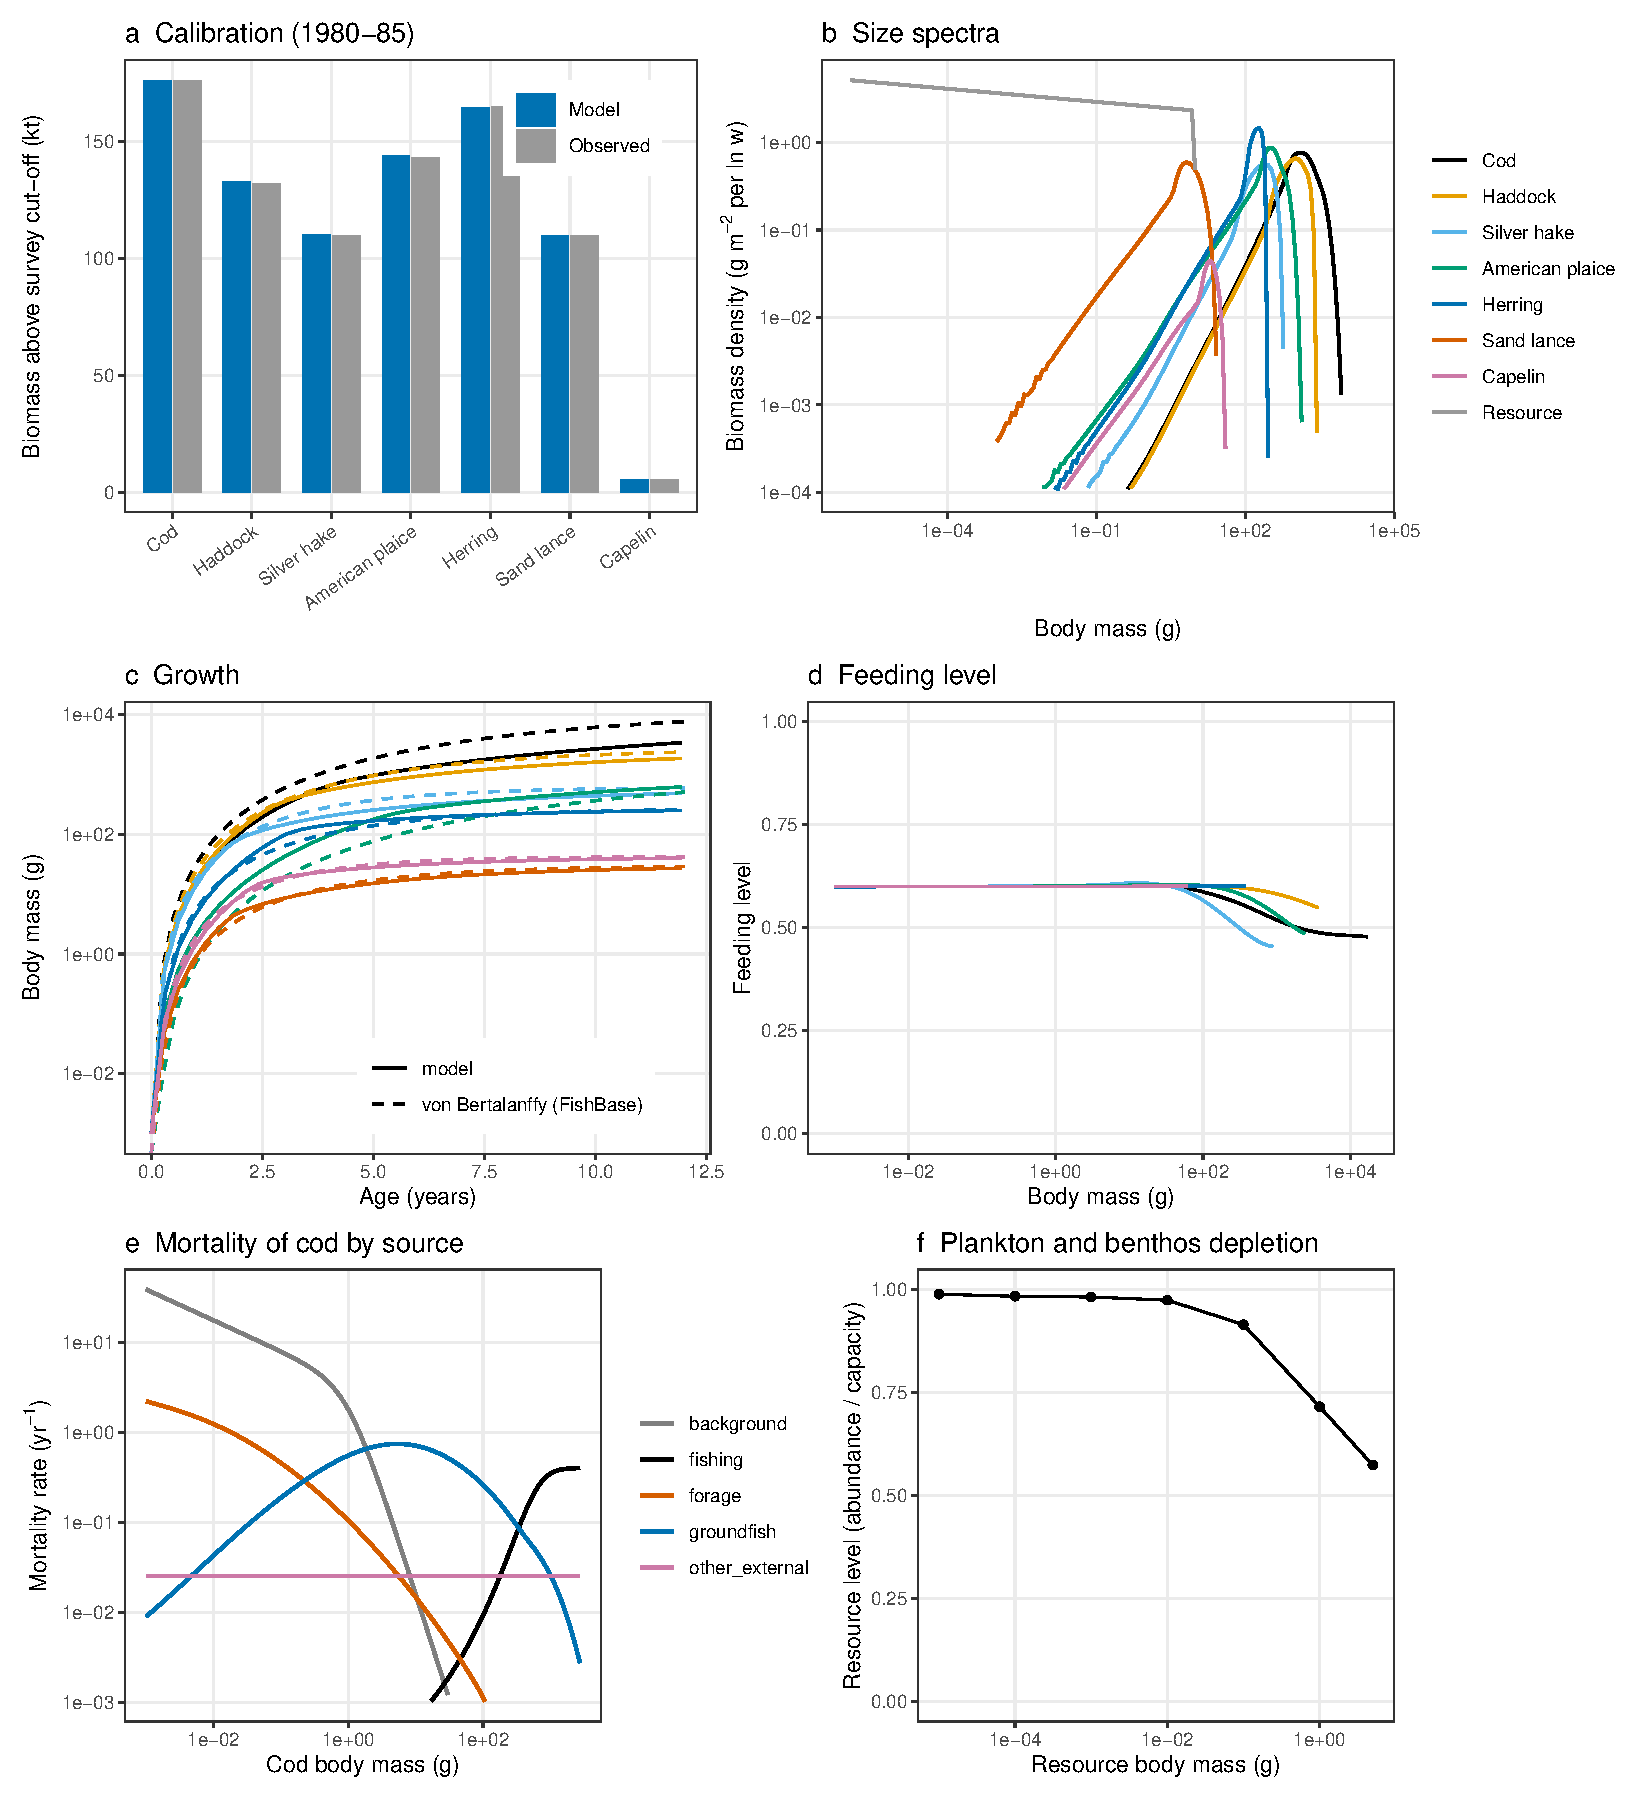
\includegraphics[width=\textwidth,height=0.82\textheight,keepaspectratio]{../figures/fig1_baseline.pdf}
\caption{The calibrated 1980--85 steady state of v3 as produced by \nolinkurl{R/01_build_model.R}: (a) biomass above the survey cut-off, model and target (kt); (b) size spectra and resource; (c) growth, model (solid) and von Bertalanffy curves from FishBase parameters (dashed); (d) feeding level; (e) mortality of cod by source; (f) resource level (abundance/capacity) by size.}\label{fig:S-baseline}\end{figure}

\begin{figure}[p]\centering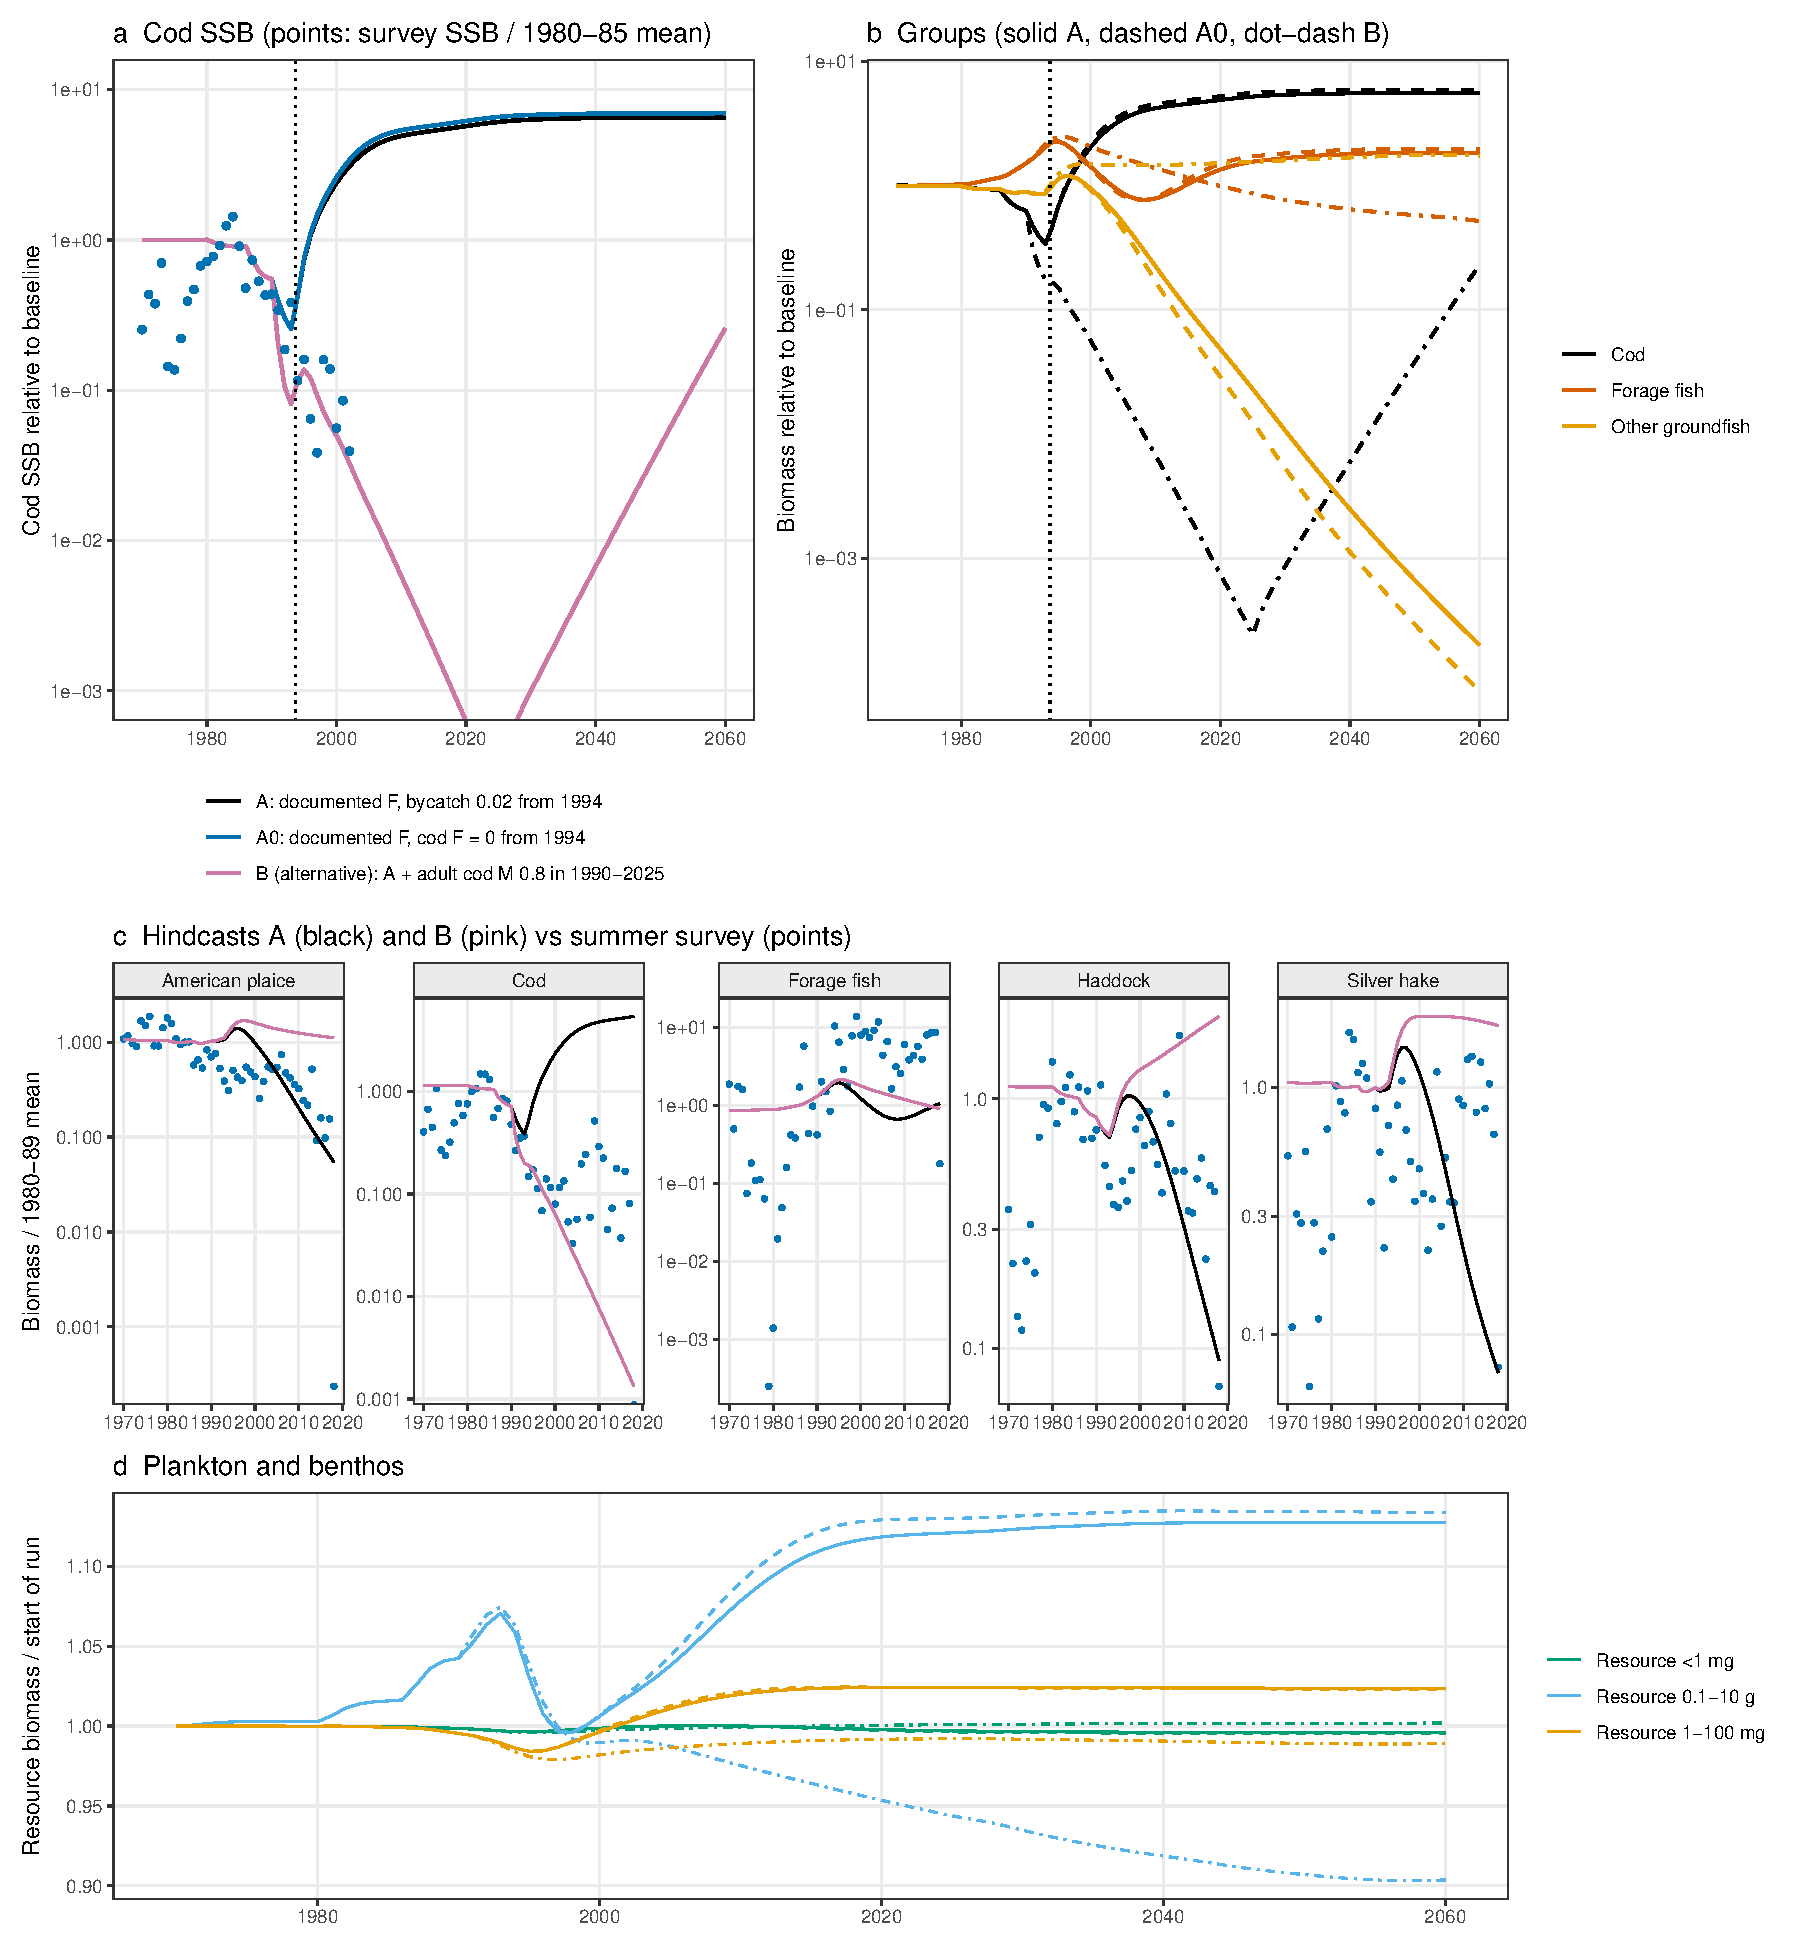
\includegraphics[width=\textwidth,height=0.82\textheight,keepaspectratio]{../figures/fig2_collapse_moratorium.pdf}
\caption{Hindcast detail (\nolinkurl{R/02_collapse_moratorium.R}): (a) cod SSB relative to baseline for runs A, A0 and B with survey-based SSB (points); (b) cod, forage fish and other groundfish relative to baseline (solid A, dashed A0, dot-dash B); (c) runs A (black) and B (pink) against the summer survey (points) by species or group, relative to 1980--89 means; (d) resource biomass in three size bands relative to the start of the run.}\label{fig:S-hind}\end{figure}

\begin{figure}[p]\centering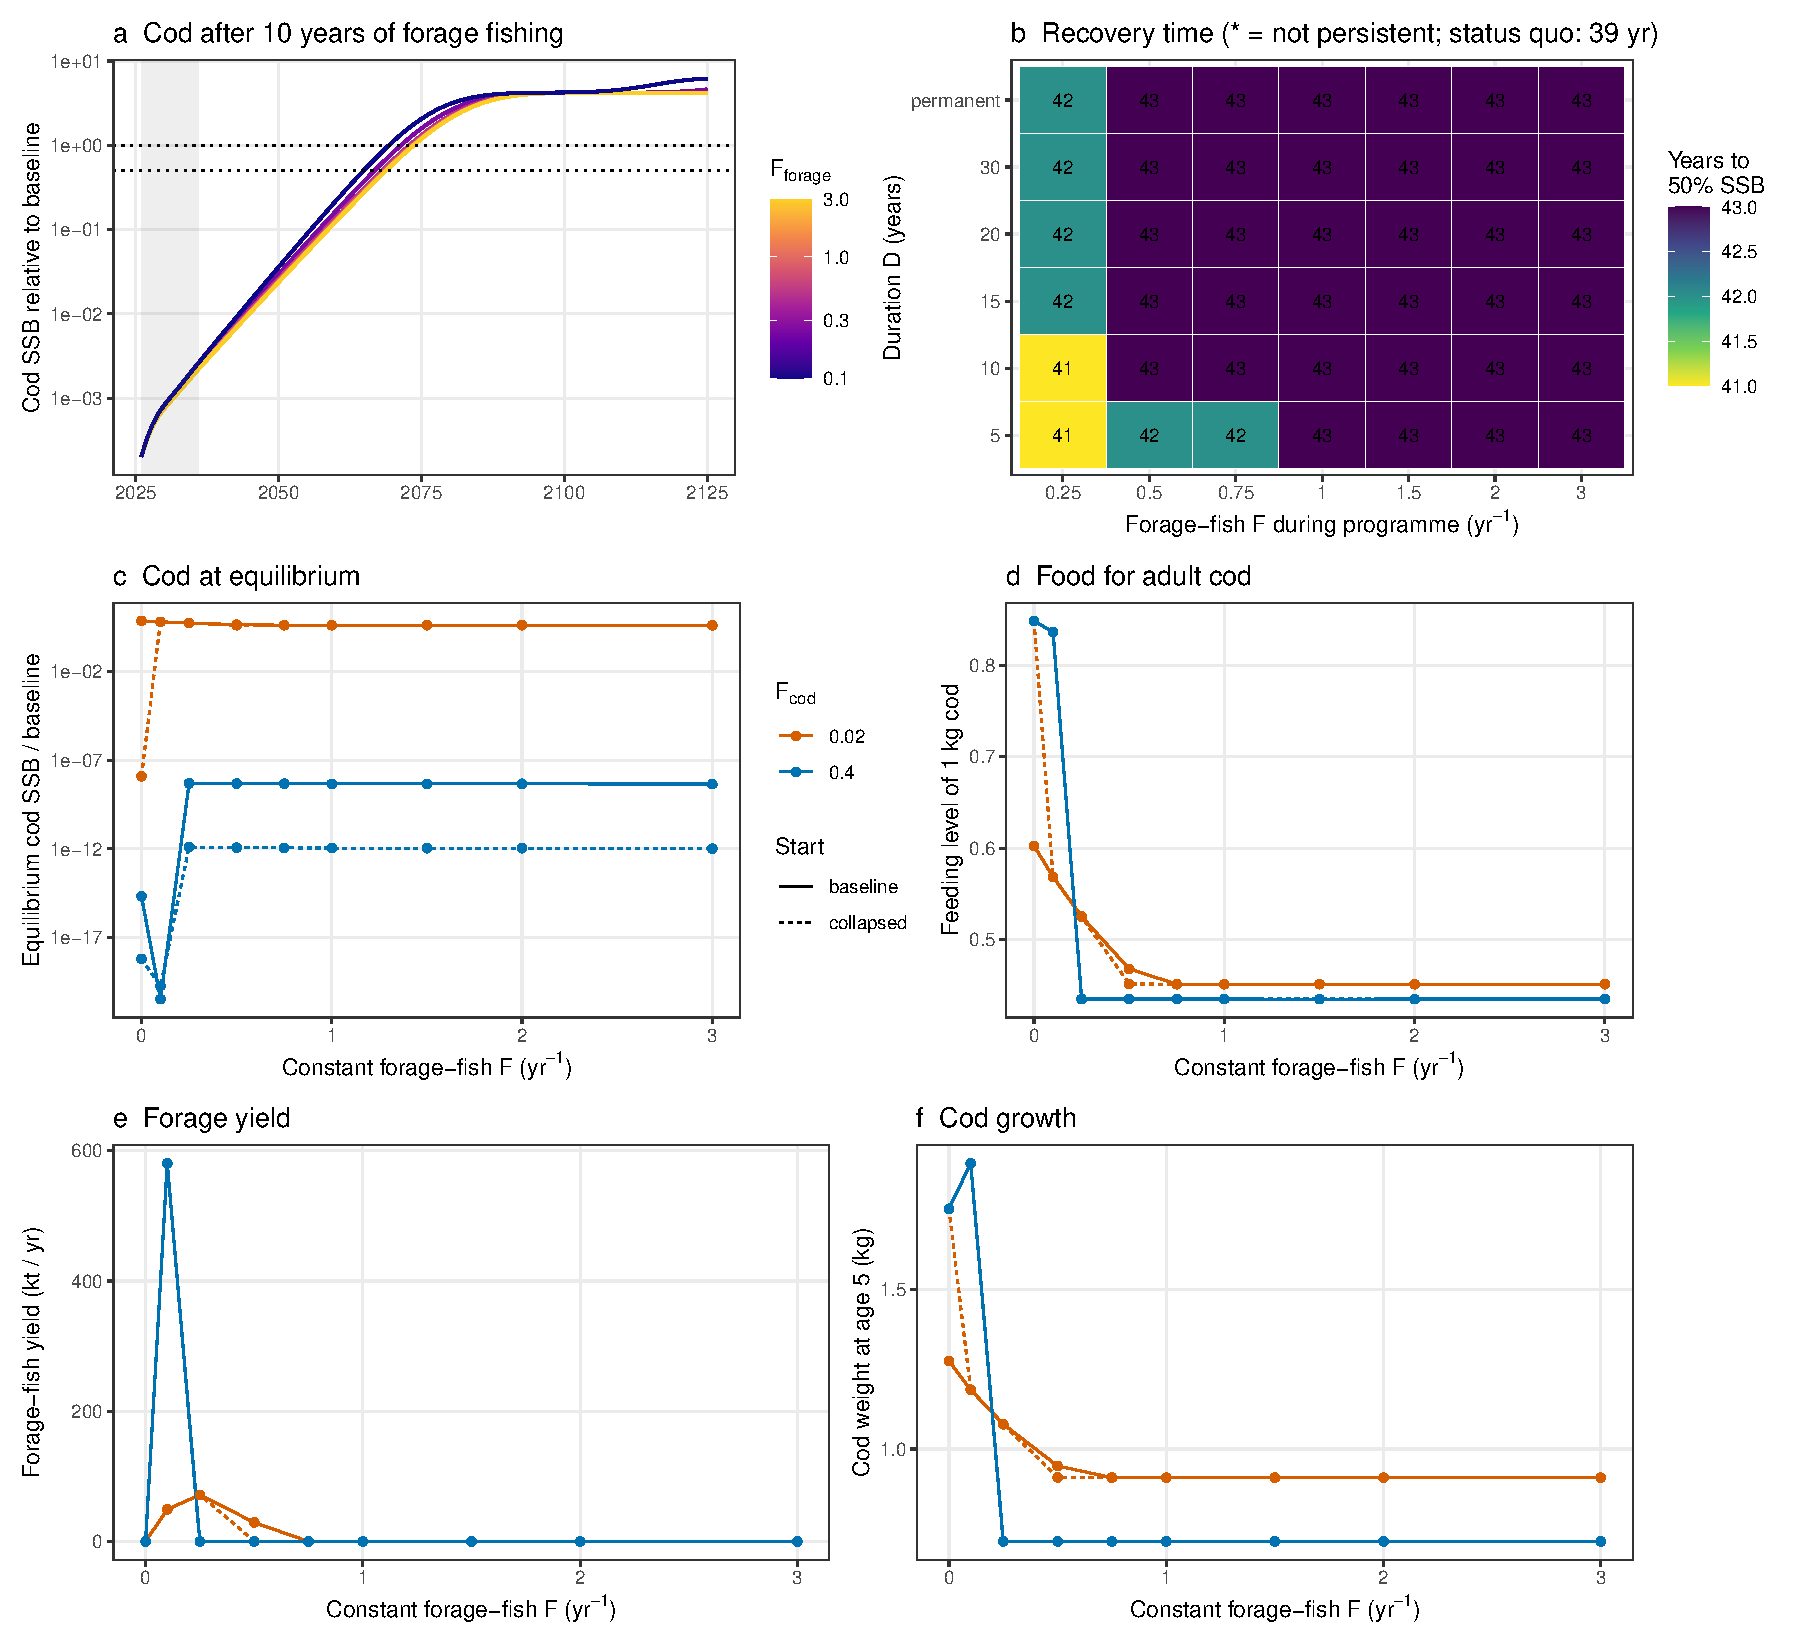
\includegraphics[width=\textwidth,height=0.82\textheight,keepaspectratio]{../figures/fig4_forage_fishing.pdf}
\caption{Forage fishing from the modelled collapsed 2025 state (\nolinkurl{R/04_forage_fishing_recovery.R}): (a) cod SSB after 10-year programmes (shaded); (b) years to 50\% of baseline SSB by forage-fish $F$ and duration (status quo 39 years); (c--f) constant-forage-$F$ equilibria with cod $F$ 0.02 (orange) or 0.40 (blue) from the baseline (solid) and the collapsed state (dotted): (c) cod SSB, (d) feeding level of 1-kg cod, (e) forage yield, (f) cod weight at age 5.}\label{fig:S-forage}\end{figure}

\begin{figure}[p]\centering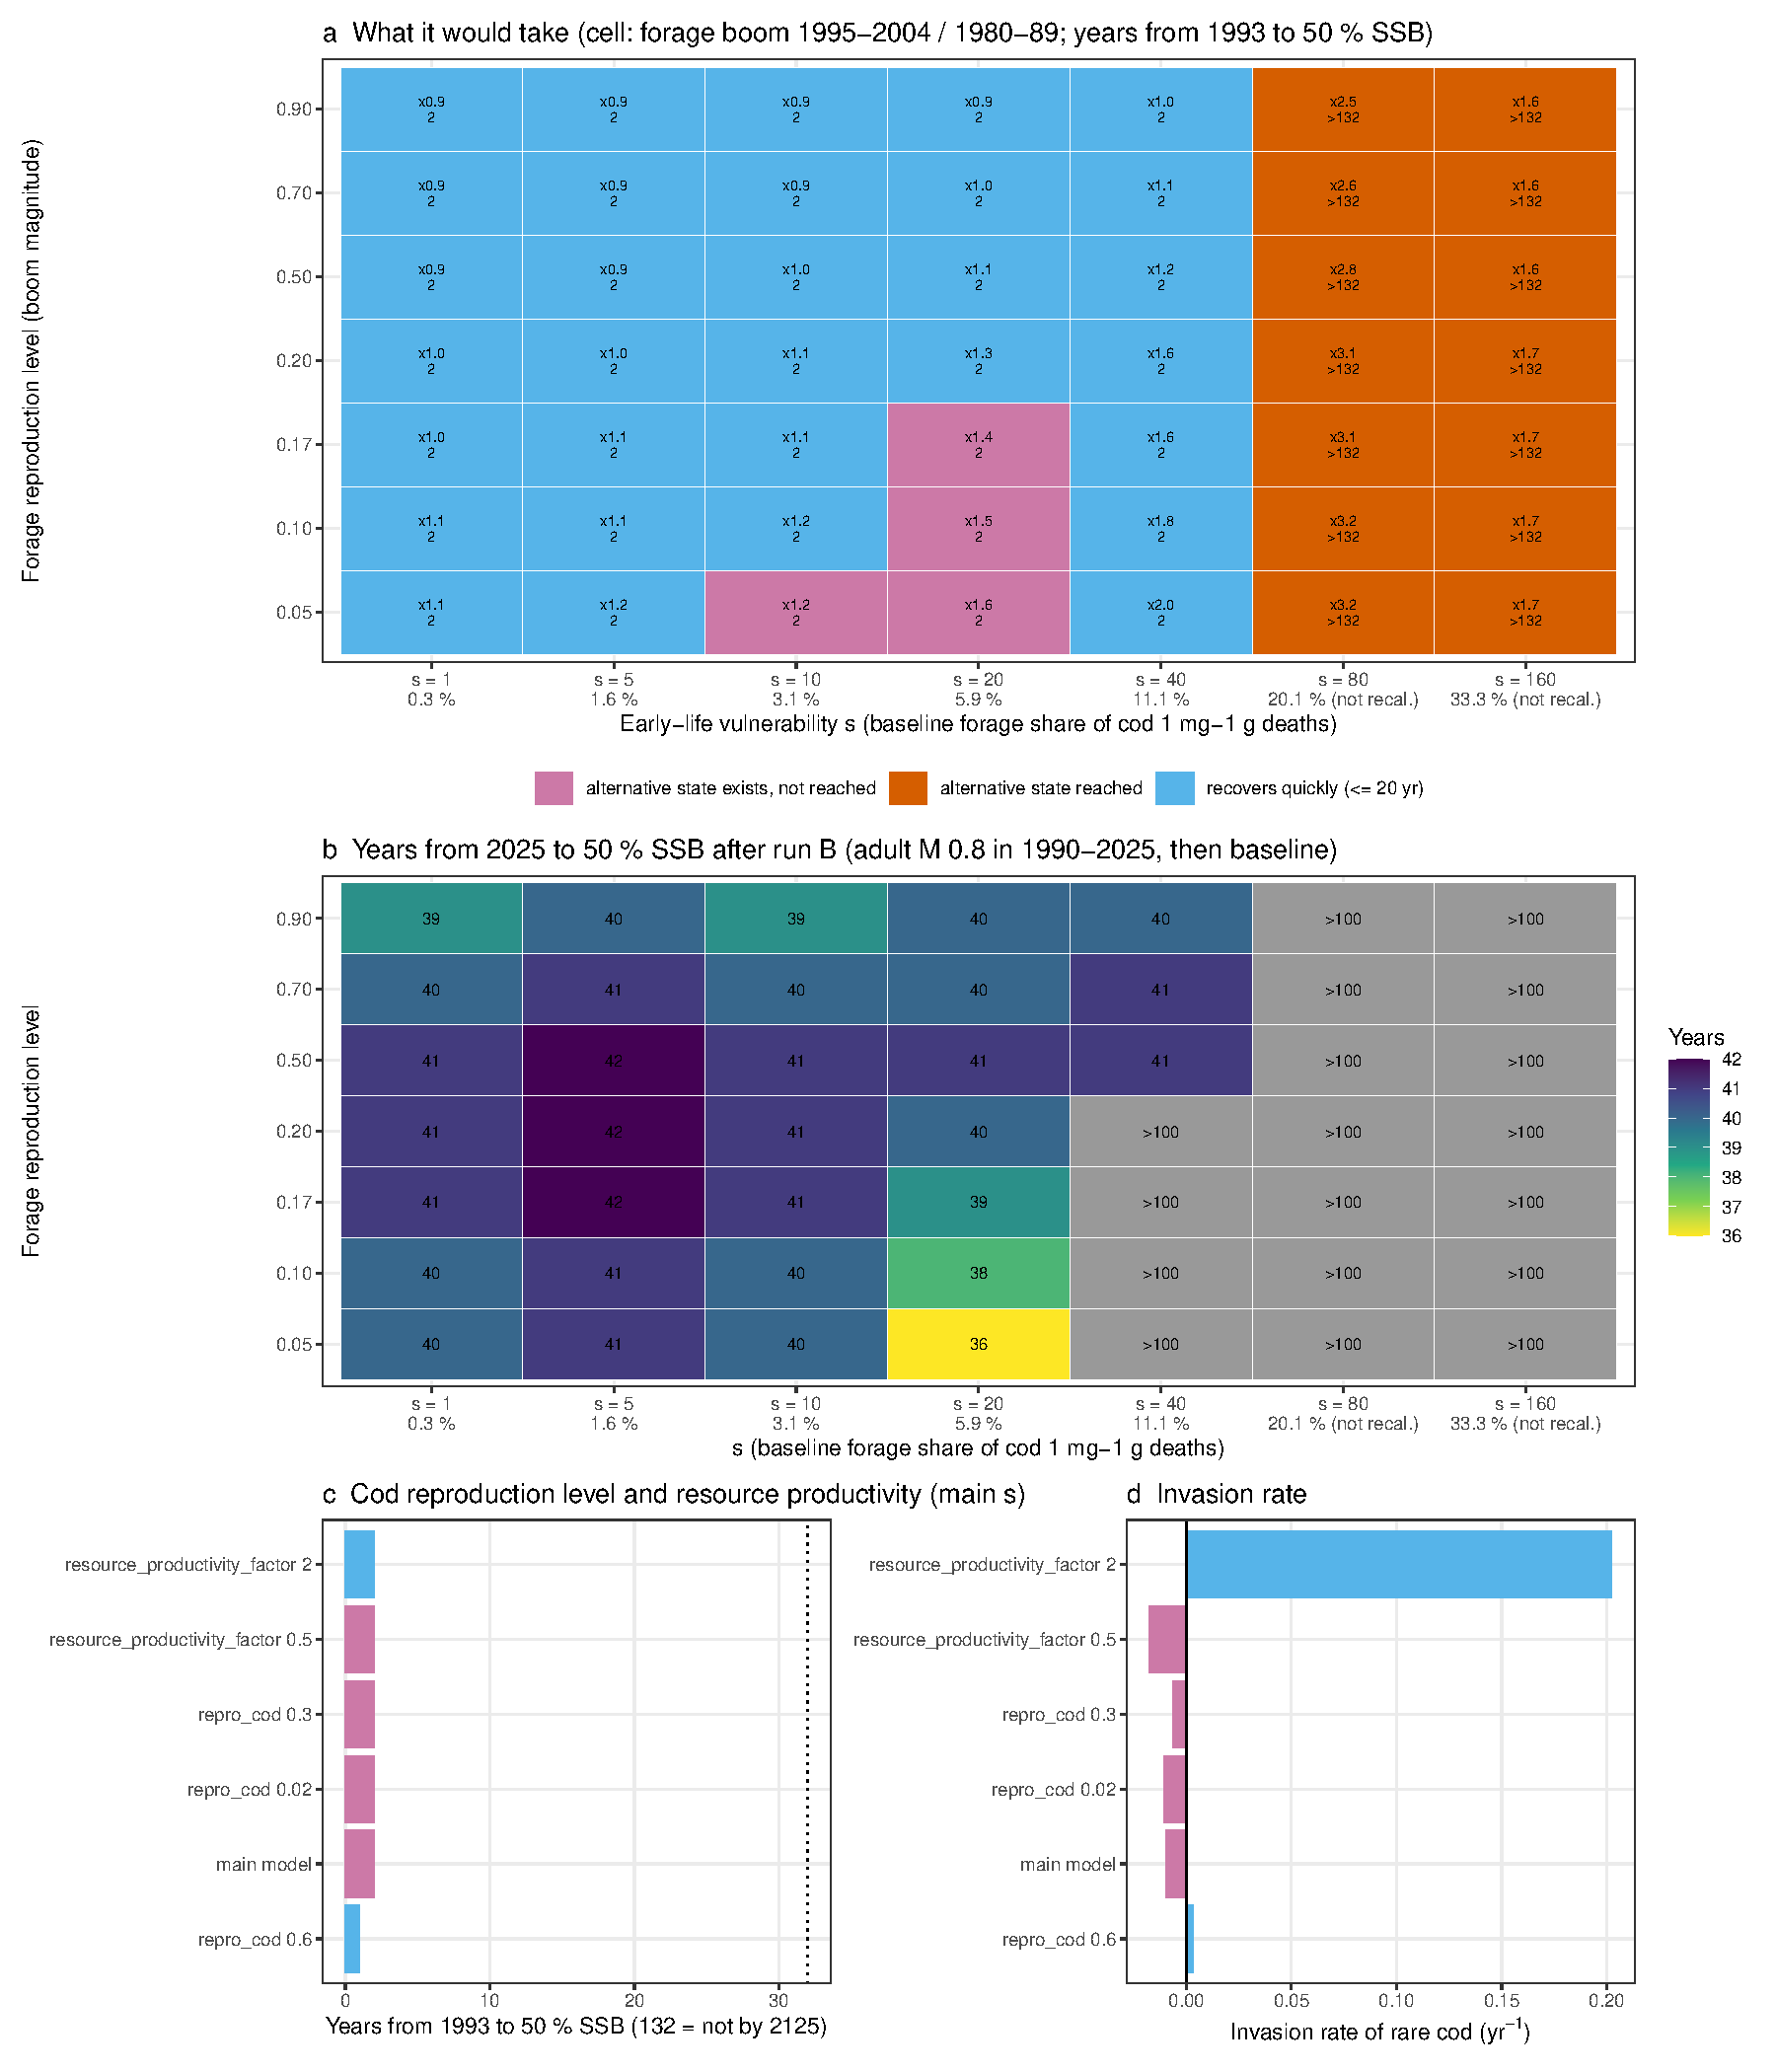
\includegraphics[width=\textwidth,height=0.82\textheight,keepaspectratio]{../figures/fig5_sensitivity.pdf}
\caption{Sensitivity analysis as produced by \nolinkurl{R/05_sensitivity.R}: (a) outcome classes over $s$ and the forage reproduction level (cell text: forage boom 1995--2004/1980--89 and years from 1993 to 50\% SSB; $>$132: not by 2125); (b) years from 2025 to 50\% SSB after run~B; (c) one-at-a-time variants at $s=20$: years from 1993 to 50\% SSB; (d) invasion rate of rare cod. Colours: blue, recovers within 20 years; pink, alternative state exists but not reached; orange, alternative state reached.}\label{fig:S-sens}\end{figure}

\begin{figure}[p]\centering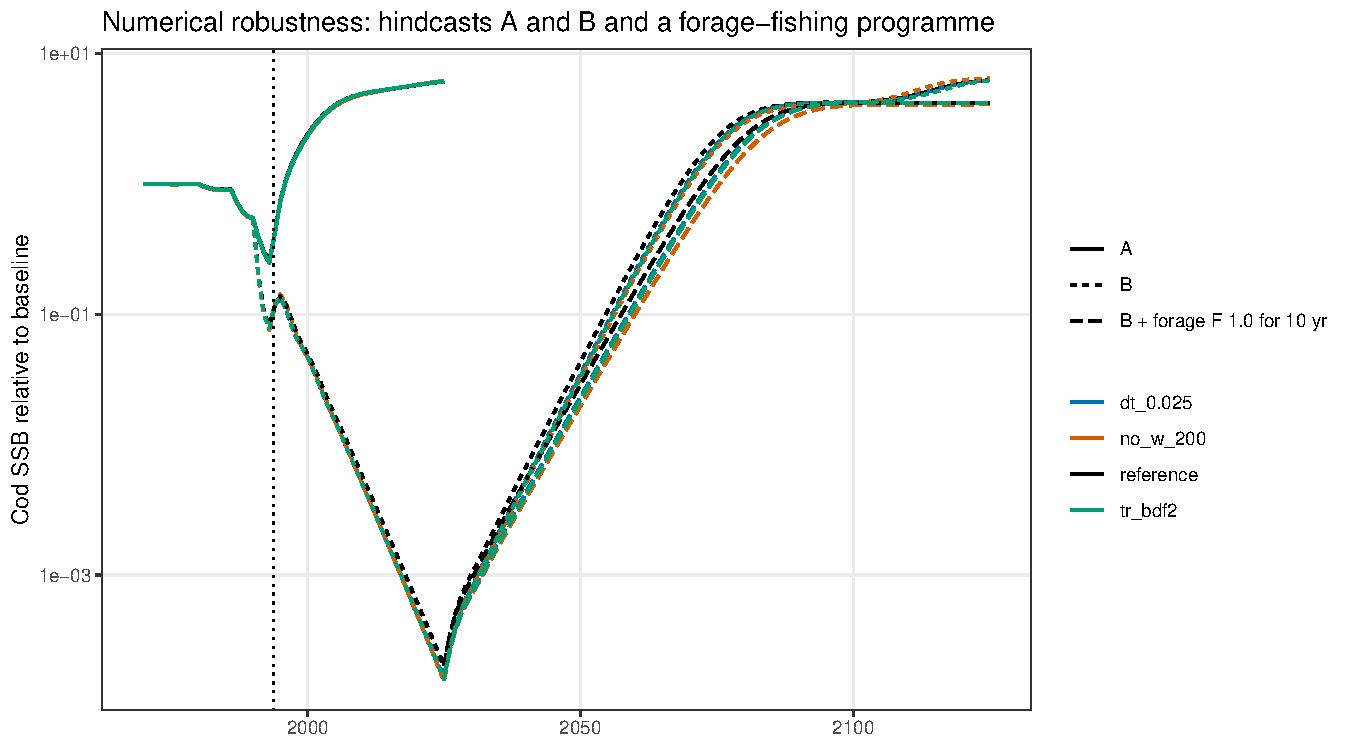
\includegraphics[width=\textwidth,height=0.82\textheight,keepaspectratio]{../figures/figS1_numerical_checks.pdf}
\caption{Numerical checks (\nolinkurl{R/06_numerical_checks.R}): cod SSB relative to baseline in run A (solid), run B (dotted) and run B followed by forage-fish $F=1$ for 10 years (dashed), with the reference numerics, a time step of 0.025~yr, TR-BDF2 time stepping and a 200-bin size grid (recalibrated).}\label{fig:S-num}\end{figure}

\begin{figure}[p]\centering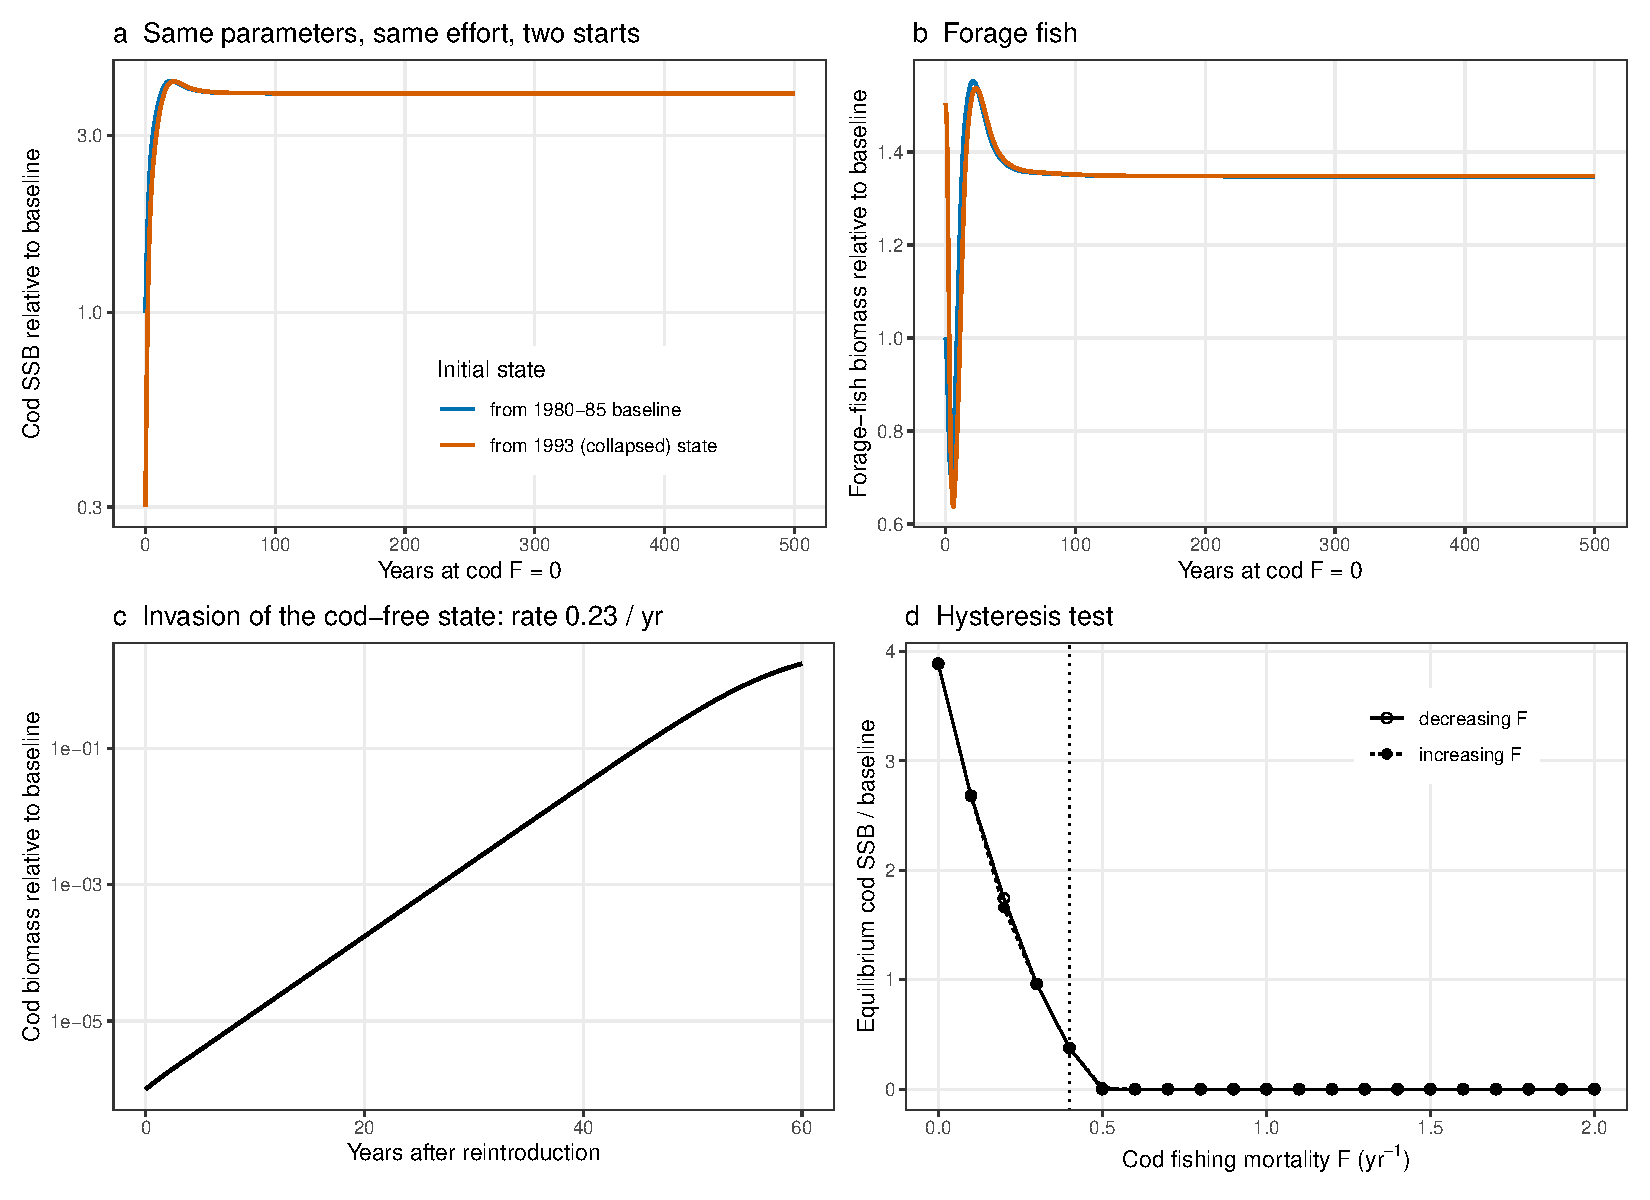
\includegraphics[width=\textwidth,height=0.82\textheight,keepaspectratio]{../figures/v1/fig3_bistability.pdf}
\caption{Model v1 ($s=1$): bistability test at cod $F=0$. (a) Cod SSB from the 1980--85 baseline and from the 1993 hindcast state; (b) forage biomass; (c) cod reintroduced into the cod-free community grows at $+0.23$~\yr{}; (d) equilibrium cod SSB against cod $F$, increasing and decreasing. No alternative state.}\label{fig:S-v1}\end{figure}

\begin{figure}[p]\centering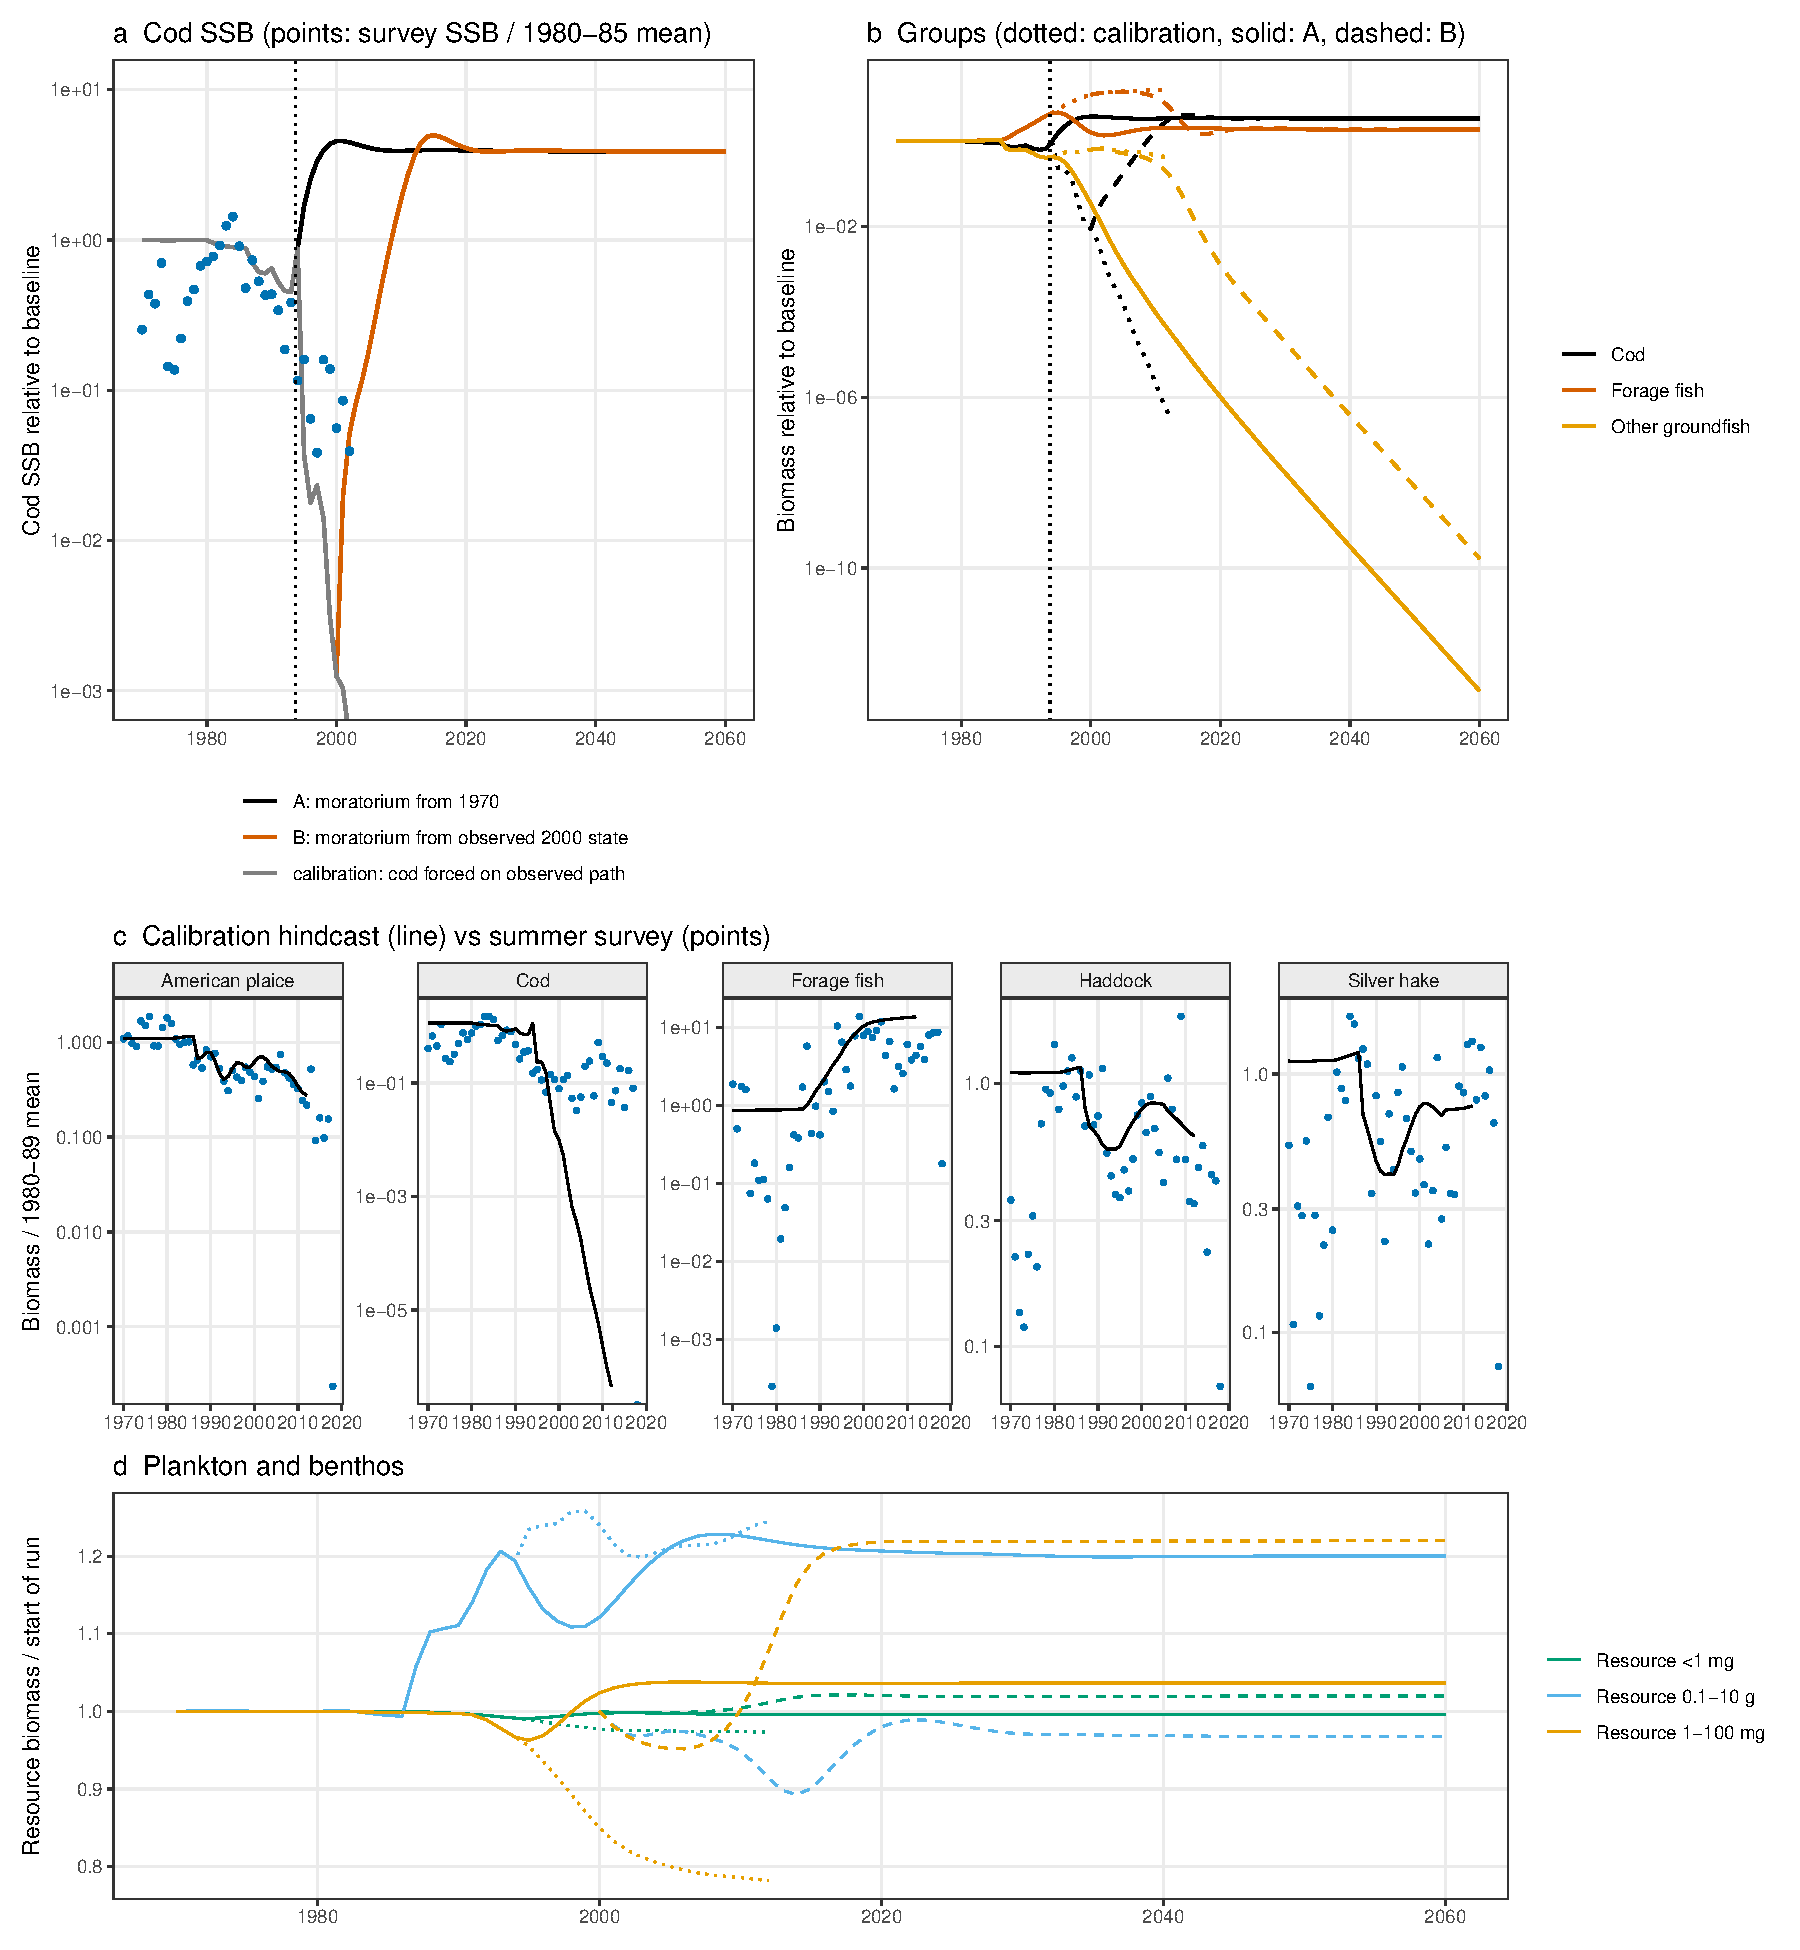
\includegraphics[width=\textwidth,height=0.82\textheight,keepaspectratio]{../figures/v2/fig2_collapse_moratorium.pdf}
\caption{Model v2 ($s=1$): (a) cod SSB in the calibration run in which cod was forced down by an effective $F$ of 6.28 from 1994 (grey), in a moratorium from 1970 (A) and in a moratorium from the model's observed-like 2000 state (B), with survey-based SSB (points); (b) groups; (c) calibration run against the summer survey; (d) resource bands. The forced run reproduces the forage boom (9.4-fold) but the boom does not fade; from the 2000 state cod regains 50\% of baseline SSB in 7 years.}\label{fig:S-v2hind}\end{figure}

\begin{figure}[p]\centering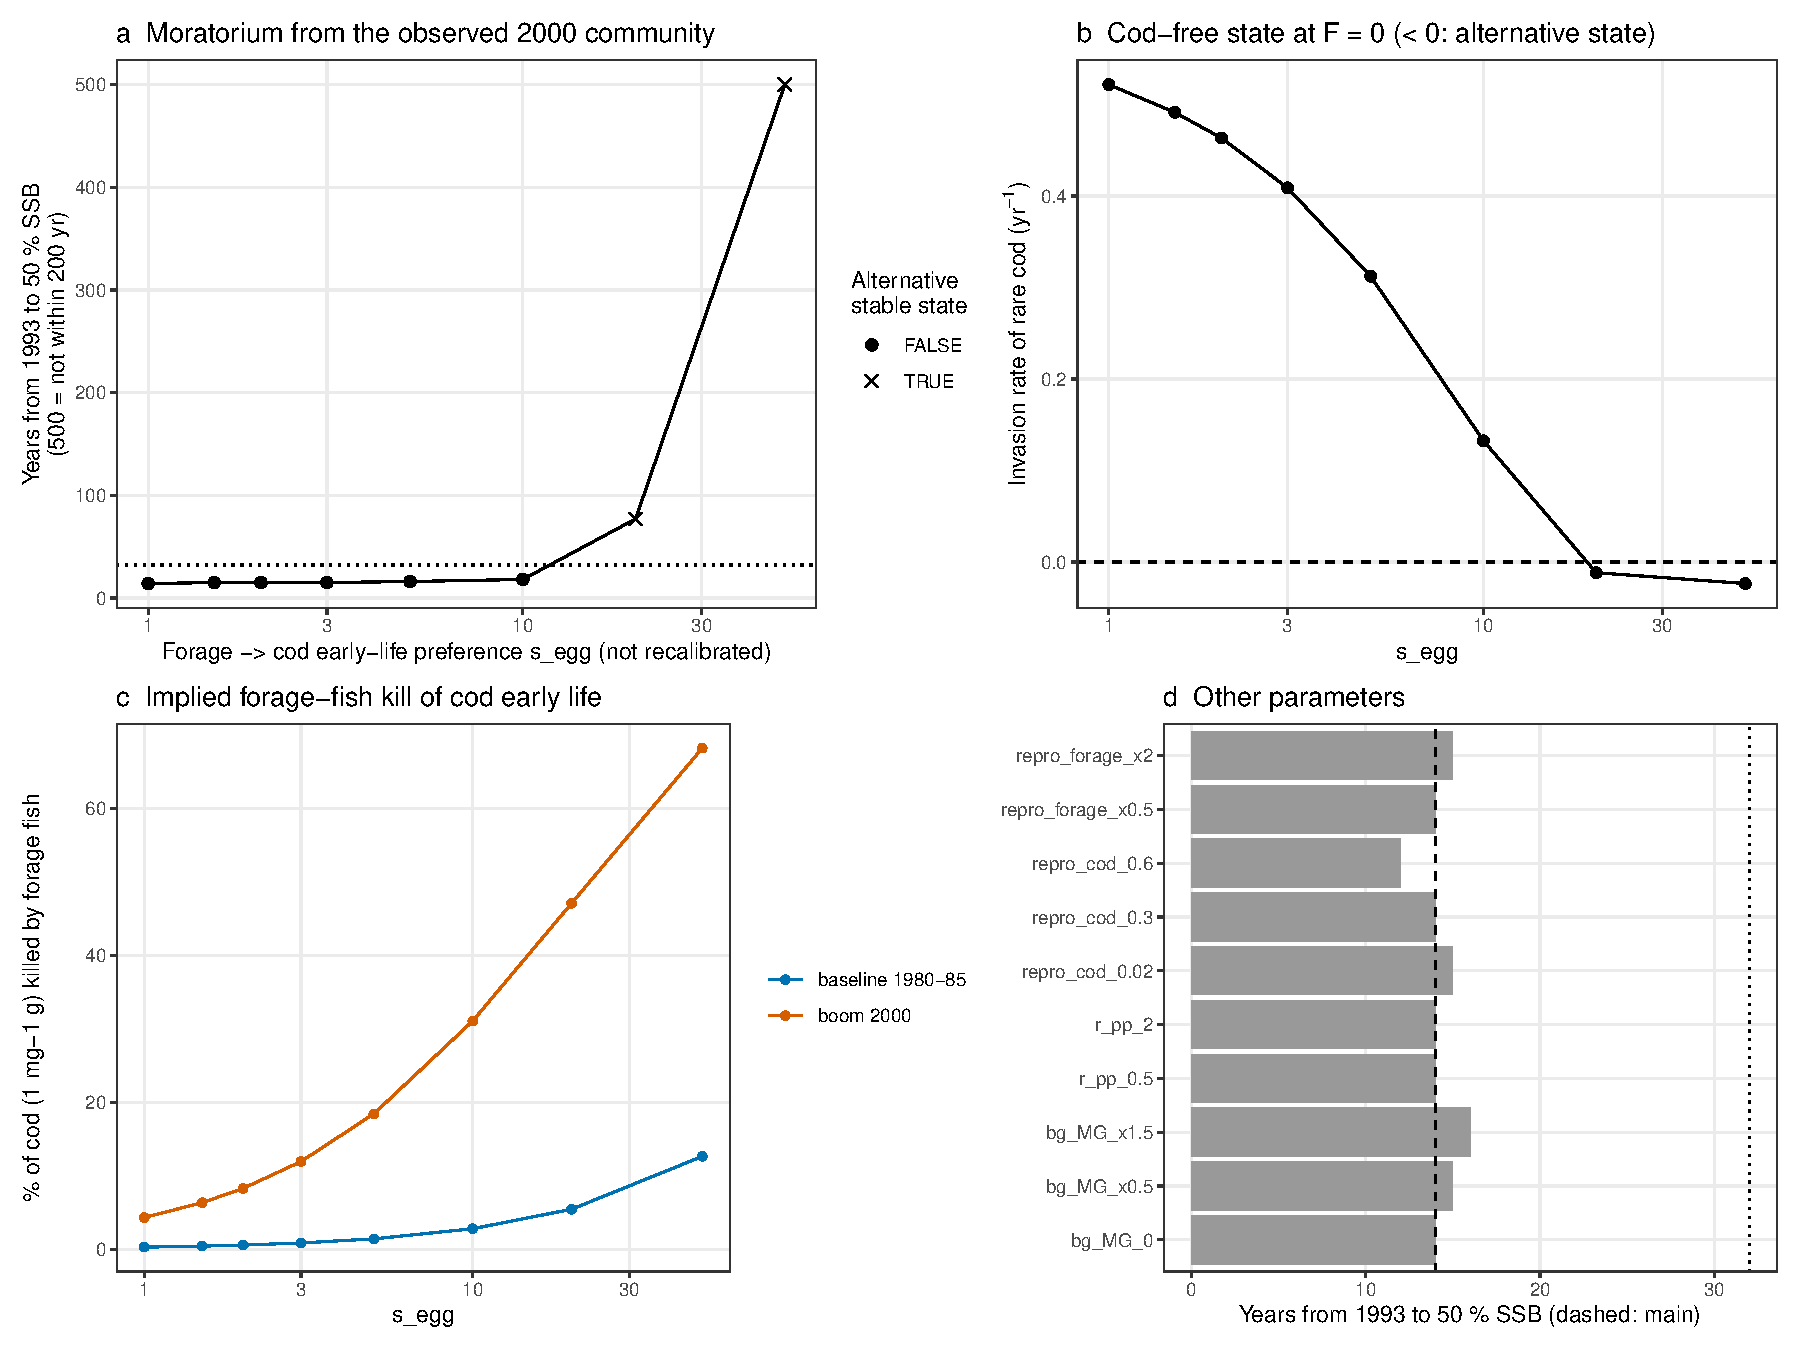
\includegraphics[width=\textwidth,height=0.82\textheight,keepaspectratio]{../figures/v2/fig5_sensitivity.pdf}
\caption{Model v2: effect of raising the forage$\rightarrow$cod early-life factor (here called $s_{\mathrm{egg}}$) without recalibration. (a) Years from 1993 to 50\% SSB after a moratorium from the observed-like 2000 state; (b) invasion rate of rare cod in the cod-free state; (c) implied percentage of cod 1~mg--1~g killed by forage fish at baseline and in the 2000 boom; (d) other parameters. Without recalibration, the 1980s cod is no longer sustained at $s_{\mathrm{egg}}\geq10$.}\label{fig:S-v2sens}\end{figure}

\end{document}
